%Version 3 December 2023
% See section 11 of the User Manual for version history
%
%%%%%%%%%%%%%%%%%%%%%%%%%%%%%%%%%%%%%%%%%%%%%%%%%%%%%%%%%%%%%%%%%%%%%%
%%                                                                 %%
%% Please do not use \input{...} to include other tex files.       %%
%% Submit your LaTeX manuscript as one .tex document.              %%
%%                                                                 %%
%% All additional figures and files should be attached             %%
%% separately and not embedded in the \TeX\ document itself.       %%
%%                                                                 %%
%%%%%%%%%%%%%%%%%%%%%%%%%%%%%%%%%%%%%%%%%%%%%%%%%%%%%%%%%%%%%%%%%%%%%

%%\documentclass[referee,sn-basic]{sn-jnl}% referee option is meant for double line spacing

%%=======================================================%%
%% to print line numbers in the margin use lineno option %%
%%=======================================================%%

%%\documentclass[lineno,sn-basic]{sn-jnl}% Basic Springer Nature Reference Style/Chemistry Reference Style

%%======================================================%%
%% to compile with pdflatex/xelatex use pdflatex option %%
%%======================================================%%

%%\documentclass[pdflatex,sn-basic]{sn-jnl}% Basic Springer Nature Reference Style/Chemistry Reference Style


%%Note: the following reference styles support Namedate and Numbered referencing. By default the style follows the most common style. To switch between the options you can add or remove “Numbered” in the optional parenthesis. 
%%The option is available for: sn-basic.bst, sn-vancouver.bst, sn-chicago.bst%  
 
%%\documentclass[pdflatex,sn-nature]{sn-jnl}% Style for submissions to Nature Portfolio journals
%%\documentclass[pdflatex,sn-basic]{sn-jnl}% Basic Springer Nature Reference Style/Chemistry Reference Style
\documentclass[pdflatex,sn-mathphys-num]{sn-jnl}% Math and Physical Sciences Numbered Reference Style 
%%\documentclass[pdflatex,sn-mathphys-ay]{sn-jnl}% Math and Physical Sciences Author Year Reference Style
%%\documentclass[pdflatex,sn-aps]{sn-jnl}% American Physical Society (APS) Reference Style
%%\documentclass[pdflatex,sn-vancouver,Numbered]{sn-jnl}% Vancouver Reference Style
%%\documentclass[pdflatex,sn-apa]{sn-jnl}% APA Reference Style 
%%\documentclass[pdflatex,sn-chicago]{sn-jnl}% Chicago-based Humanities Reference Style

%%%% Standard Packages
%%<additional latex packages if required can be included here>
\usepackage{lineno}
\usepackage{graphicx}%
\usepackage{multirow}%
\usepackage{amsmath,amssymb,amsfonts}%
\usepackage{amsthm}%
\usepackage{mathrsfs}%
\usepackage[title]{appendix}%
\usepackage{xcolor}%
\usepackage{textcomp}%
\usepackage{manyfoot}%
\usepackage{booktabs}%
\usepackage{algorithm}%
% \usepackage{algorithmicx}%
\usepackage{algorithmic}
\renewcommand{\algorithmicrequire}{\textbf{Input:}}
\renewcommand{\algorithmicensure}{\textbf{Output:}}
% \usepackage{algpseudocode}%s
\usepackage{listings}%
\usepackage{float}
\usepackage{tcolorbox}
%%%%

%%%%%=============================================================================%%%%
%%%%  Remarks: This template is provided to aid authors with the preparation
%%%%  of original research articles intended for submission to journals published 
%%%%  by Springer Nature. The guidance has been prepared in partnership with 
%%%%  production teams to conform to Springer Nature technical requirements. 
%%%%  Editorial and presentation requirements differ among journal portfolios and 
%%%%  research disciplines. You may find sections in this template are irrelevant 
%%%%  to your work and are empowered to omit any such section if allowed by the 
%%%%  journal you intend to submit to. The submission guidelines and policies 
%%%%  of the journal take precedence. A detailed User Manual is available in the 
%%%%  template package for technical guidance.
%%%%%=============================================================================%%%%

%% as per the requirement new theorem styles can be included as shown below
\theoremstyle{thmstyleone}%
\newtheorem{theorem}{Theorem}%  meant for continuous numbers
%%\newtheorem{theorem}{Theorem}[section]% meant for sectionwise numbers
%% optional argument [theorem] produces theorem numbering sequence instead of independent numbers for Proposition
\newtheorem{proposition}[theorem]{Proposition}% 
%%\newtheorem{proposition}{Proposition}% to get separate numbers for theorem and proposition etc.

\theoremstyle{thmstyletwo}%
\newtheorem{example}{Example}%
\newtheorem{remark}{Remark}%

\theoremstyle{thmstylethree}%
\newtheorem{definition}{Definition}%

\raggedbottom
\linenumbers
%%\unnumbered% uncomment this for unnumbered level heads

\begin{document}

\title[Article Title]{An Agent-Oriented Framework to Support Rapid Early-Stage Object-Oriented Design}

\author*[1]{\fnm{Yilong} \sur{Yang}}\email{yilongyang@buaa.edu.cn}
\author[1]{\fnm{Runkun} \sur{Zhang}}\email{runkunzhang@buaa.edu.cn}
\author[1]{\fnm{Zhen} \sur{Tian}}\email{zhentian1@buaa.edu.cn}
\author[2]{\fnm{Weiru} \sur{Wang}}\email{weiru.wang@bjut.edu.cn}
% \equalcont{These authors contributed equally to this work.}

\affil[1]{\orgdiv{School of Software}, \orgname{Beihang University}, \orgaddress{\city{Beijing}, \postcode{100191}, \country{China}}}
\affil[2]{\orgdiv{College of Computer Science}, \orgname{Beijing
University of Technology}, \orgaddress{\city{Beijing}, \postcode{100083}, \country{China}}}
% \affil[2]{\orgdiv{Department}, \orgname{Organization}, \orgaddress{\street{Street}, \city{City}, \postcode{10587}, \state{State}, \country{Country}}}

\abstract{% 面向对象（OO）设计是软件工程中的基石方法论，在当代软件开发中扮演着关键角色。然而，制作有效的面向对象设计模型需要密集的心智努力和复杂的专业知识。尽管现有的需求建模研究已经相当全面，涵盖了从自然语言处理或手工构建获取需求模型的方法，以及自动原型设计助于迅速验证这些模型，但通过自动化精细化从需求生成设计模型的自动化生成代表了一个减少设计阶段努力的有希望的途径。

% 在本文中，我们引入了一种名为RapidOOD的面向Agent的集成了模型驱动和LLMs的方法论，旨在通过促进从验证的需求模型生成、评估和优化OO设计模型来减轻软件开发挑战。我们开发了一个工具来自动化这一方法论。我们基于六个现有需求模型的评估表明，类图元素的全部和顺序图元素的94.8%可以在10秒内准确生成。自动生成的并随后优化的设计模型与手工制作的模型在质量上紧密匹配。此外，我们的方法展示了与手工软件设计师组相比，在包括为正式需求模型中的OCL契约建模时间在内，可以减少28.1%的时间成本。

% 总体而言，研究结果是有希望的，表明RapidOOD可以进一步完善并应用于行业系统开发中。
Object-Oriented (OO) design, as a cornerstone methodology in software engineering, has been
playing a pivotal role in software development, during which OO design models are often crafted. 
However, the challenge is always on intensive cognitive effort and expertise required for modeling. 
% While existing research on requirements modeling is comprehensive, 
% covering requirements model derivation from natural language processing or manual construction, 
% and auto-prototyping aids in swiftly validating these models, 
In the past, automatically generating models from requirements has been considered a promising direction to overcome this challenge. The model-driven engineering \textcolor{red}{(MDE)} community has intensively made effort towards this direction. Though some progresses have been made with the help of natural language processing (NLP) techniques, fully automated solutions are rare due to the limitation of NLP techniques themselves, and generated models are not full correct and/or complete. Towards this direction, in this paper, we introduce an agent-oriented methodology with tool support, named RapidOOD, which leverages large language models (LLMs) for the generation, quality assessment, and refactoring of OO design models, by taking requirements models as the input. Our evaluation of RapidOOD with six requirement models demonstrates that automatically generated and subsequently optimized design models achieve 89.20\% (without human) and 94.56\% (human-in-the-loop collaboration) of expert-level quality metrics, closely matching models crafted manually by experts. Furthermore, our approach achieves 1.39 times the efficiency of the manual method.% Furthermore, our approach shows a 28.1\% reduction in time cost.%, including modeling time for OCL contracts in formal requirements models, compared to the manual software designers group.
%Overall, the findings are promising, suggesting that RapidOOD can be further refined and applied within industry systems development.
}


% \keywords{Object-Oriented, Software Design, Model Driven Architecture, Agent-Oriented}
\keywords{Object-Oriented, Agent-Oriented, Model Generation, Model Refactoring, Large Language Model}

\maketitle

\section{Introduction}\label{sec1}

% 软件设计是软件开发的基础部分，包括两个主要阶段:架构设计和详细设计。优秀的软件设计对于生产高质量的软件至关重要。面向对象的设计方法可以在设计过程中创建不同的抽象类型，比面向过程的设计方法更直观，受到了广泛的关注。经过几十年的发展，面向对象的思想已经在软件工程中根深蒂固，现在已经成为主流的软件设计和开发方法之一。
% \cite{Design1} A.H. Eden and R. Kazman. 2003. Architecture, design, implementation. In 25th International Conference on Software Engineering, 2003. Proceedings. 149–159
Software design is a fundamental part of software development, covering two primary stages: architectural design and detailed design\cite{Design1}. The object-oriented design method, which facilitates the creation of different abstract types during the design process, is more intuitive than the process-oriented design method and has garnered considerable attention. After decades of evolution, object-oriented design has become one of the main approaches to software design and development\cite{flageol_mapping_2023}.
% 利用模型是软件设计中一项重要的辅助技术。由于文本描述在开发、评审和维护方面具有挑战性，因此通过图形化建模语言进行抽象可以增强客户和开发人员之间的沟通，支持需求验证，促进体系结构和详细设计，帮助原型设计，支持代码生成，等等。
% 使用统一建模语言(UML)，可以将需求建模为一个轻量级的形式化需求模型，该模型由用例图、概念类图、由系统顺序图指定的用例定义以及它们的系统操作的契约\cite{RM1, RM2, RM3}，组成。在对象约束语言(OCL)中，系统操作契约由一对前置条件和后置条件形式化地描述。设计可以使用类图和序列图进行建模。工作在需求阶段，如RM2PT \cite{YangICSE19, YangRE, YangTR, RM2Doc}提供了用于需求建模、分析和从需求模型自动生成原型的功能。用户可以通过RM2PT快速验证和演化功能需求，从而产生高质量的验证需求模型。验证过的需求模型可以作为设计阶段的输入。
Utilizing models is a vital supplementary technique in software design. 
Since textual descriptions are challenging to employ for development, review, and maintenance, abstraction through graphical modeling languages is used to enhance communication between customers and developers, support requirements validation, facilitate architectural and detailed design, aid in prototyping, enable code generation, and more. 
With Unified Modeling Language(UML), requirements can be modeled as a lightweight formal requirements model that consists of a use case diagram, a conceptual class diagram, use case definitions specified by system sequence diagrams, and the contracts of their system operations\cite{RM1, RM2, RM3}. 
A system operation contract is formally specified by a pair of pre- and post-conditions in Object Constraint Language (OCL). 
Designs can be modeled using class diagrams and sequence diagrams. 
Works in requirements phase like RM2PT\cite{YangICSE19, YangRE, YangTR, RM2Doc} provides features for requirements modeling, analysis, and automated prototype generation from requirements models. 
Users can rapidly validate and evolve functional requirements through RM2PT to produce high-quality validated requirements models. 
The validated requirements model can be used as input to the design phase.

% 软件的面向对象设计的是一项知识和精力密集的活动，设计人员需要投入大量的时间和精力为给定需求构建一个合适的设计方案。面对不同的场景和需求，需要采用不同的设计方案以及权衡考虑，这往往依赖于设计人员的经验和主观判断。并且，设计的好坏在项目早期阶段难以得到快速有效的评估。

% 本文希望通过自动化方法，减少软件设计阶段的时间和精力成本，减少对设计人员水平的依赖，并在项目早期以量化、可理解的方式反映设计质量。
Object-oriented design in software development is a knowledge and effort-intensive activity. Designers must invest significant time and effort to create an appropriate design solution for given requirements. Different scenarios and requirements necessitate different design solutions and trade-offs, often depending on the designer's experience and subjective judgment. Additionally, evaluating the design quality early in the project is challenging and usually not feasible. 

This paper aims to reduce the time and effort required during the software design phase through automated methods, lessen the dependence on the designer's expertise, and provide a quantifiable and comprehensible way to reflect design quality early in the project. The main difficulties and challenges in generating design from requirements and subsequently evaluating and optimizing the initial design include:
\begin{enumerate}
    \item \textcolor{red}{Requirements capture stakeholders' needs, goals, and desired system behaviors. In our context, we focus on functional requirements specified through lightweight formal models,} while design describes system's internal implementation. Design is a concretization and refinement of requirements, containing more detailed information. It is challenging to supplement the missing information needed to transition from requirements to design.
    \item Contracts describe the system state constraints before and after executing operations. Key challenges include determining whether there is a mapping from system states to system implementations (combinations of OO basic operations) and how to map these into operation sequences automatically.
    \item In practice, design often requires multiple iterations of quality assessment and refactoring. A critical challenge is adopting suitable iteration strategies and methods to ensure iterations progress toward improved design.
\end{enumerate}

These challenges highlight the complexity of software design, underscoring the potential benefits of automating certain aspects of the design process to improve efficiency, quality, and adaptability to changing technological trends.

% 提出了一种支持面向对象设计快速生成、评估和优化的模型驱动方法RapidOOD。RapidOOD以轻量级的形式化需求模型\cite{LWFM1}作为输入，自动生成初始的面向对象设计模型，并基于模型元素计算设计质量度量。它基于这些质量指标提供了简单的优化建议。设计师可以参考质量指标和优化建议迭代设计模型，其中每次修改对设计质量的影响都立即反映在指标上。通过自动生成、评估和优化建议，可以快速实现相对高质量的设计。
% 该方法的核心思想是，在相似类型的软件项目中，初始软件设计基于相同的架构设计原则，可以嵌入到自动化方法中。在此基础上，建立需求元素与设计元素之间的映射关系，得到初始设计模型。目前，RapidOOD主要适用于使用Java EE、Spring MVC等流行Java开发框架开发的web服务项目，因为这些项目通常采用MVC架构设计模式，这也是RapidOOD生成的初始设计所遵循的架构设计模式。
This paper presents an agent-oriented methodology named RapidOOD. 
It supports the rapid generation, quality assessment, and refactoring of object-oriented designs. 
This methodology integrates model-driven rule-based agents and LLMs Agents. 
RapidOOD takes lightweight formal requirement models\cite{LWFM1} as input, automatically generates initial object-oriented design models, and computes design quality metrics based on the model elements. 
It can offer simple rule-based refactoring suggestions based on these quality metrics, and it is also capable of providing complex refactoring recommendations based on LLMs. Designers can iterate on the design model regarding the quality metrics and refactoring suggestions, where each modification's impact on design quality is immediately reflected through the metrics. A relatively high-quality design can be quickly achieved by automating generation, quality assessment, and refactoring suggestions.
% The core idea of this method is that, in software projects of similar types, the initial software design is based on the same architectural design principles, which can be embedded into the automation method. On this basis, a mapping relationship between requirement elements and design elements can be established to obtain the initial design model. RapidOOD is primarily applicable to web service projects developed with popular Java development frameworks such as Java EE and Spring MVC because these projects typically adopt an anemic architecture design pattern, which is also the architectural design pattern followed by the initial designs generated by RapidOOD. 
% Considering the initial designs mentioned above exhibit similar architectures, it is feasible to generate the initial designs using a model-driven, rule-based Agent. The rule-based method can effectively guarantee the traceability between requirements and designs, while avoiding the unreliability caused by the hallucinations introduced by the premature use of LLMs. In the subsequent quality assessment and refactoring iterations, LLMs Agents are introduced to produce more sophisticated refactoring suggestions. These suggestions are then validated, and the models are revised by human within the iterative loop.
% 我们已经开发了一个工具来实现方法的自动化。使用6个现有的需求模型对方法进行了评估。在设计模型的生成方面，主要对提出的规则的覆盖度进行评估，评估结果由成功生成的类图和顺序图的比率表示。评估了自动生成的设计模型的质量以及经过少数迭代后的设计模型的质量相较于手动构建的模型质量的情况。评估了采用该方法的时间节省的情况。总体实验结果是令人满意的。

We have developed a tool to automate the method. This method was evaluated using six requirement models. In terms of generating design models, the main focus was on assessing the coverage of the proposed rules, with the quality assessment results represented by the ratio of successfully generated class diagram elements and sequence diagram elements. The quality of the automatically generated design models and the quality of the design models after a few iterations were evaluated against the quality of models manually constructed by experts. The time savings achieved by adopting this method were assessed on the six cases. Overall, the experimental results were satisfactory.

% 论文贡献如下: 
% \begin{enumerate}
% \item \textit{模型驱动的快速设计生成和迭代工作流:}提出了一种基于“生成-评估-优化”范式的工作流，通过自动生成设计模型、设计质量评估和优化建议，支持面向对象设计的快速生成和迭代。该工作流程为软件设计提供了新的视角和方法。
%     \item \textit{面向对象设计模型的自动生成:}本文介绍了一种从遵循贫血模型体系结构原则的需求模型直接生成面向对象设计模型以及对给定的OCL合约，分析其可执行性及合理的实现路径的自动方法。该方法有效地弥合了需求和设计之间的鸿沟，为面向对象的软件设计提供了一条高效、自动化的途径。
% \item \textit{早期设计质量评估与优化:}利用模型驱动的方法，将设计质量评估从传统的基于代码的评估推进到基于模型的评估框架。这一重大转变使在项目的初始阶段自动评估设计质量和交付优化建议成为可能。

% \end{enumerate}
The contributions of the paper are as follows: 
\begin{enumerate}
     \item \textbf{An Agent-Oriented Approach that Integrates Model-Driven Rule-Based Agents and LLM Agents:} This paper presents an agent-oriented methodology which facilitates the rapid generation, assessment, and refactoring of object-oriented designs. This methodology combines model-driven rule-based agents and LLM agents. The software design process is partitioned into an initial design phase featuring low degrees of freedom, an quality assessment phase, and an refactoring phase with high degrees of freedom. During the phases with low degrees of freedom, rule-based Agents are utilized to avoid problems like hallucinations resulting from the premature application of LLMs. In the phases with high degrees of freedom, LLMs are incorporated to fully exploit their knowledge-emergence capabilities.
    \item \textbf{A Method for Analyzing the Executability of OCL Contracts and Path Reasoning:} Our work introduces an automated approach for analyzing the executability of a given OCL contract and determine a reasonable implementation path. This method effectively bridges the gap between requirements and design, providing an efficient, automated pathway for object-oriented software design.
    \item \textbf{Design refactoring with Embedding quality assessment Results in LLM Prompts:} Utilizing a model-driven methodology, this research advances design quality quality assessment from code-based assessments to an innovative model-based framework. The design quality quality assessment results obtained through the model-driven method are embedded into LLM Prompts to guide the LLM to propose corresponding refactoring suggestions
   
\end{enumerate}

The rest of this article is organized as follows. Section 2 discusses the related work. Section 3 presents the background of our approach. Section 4 introduces RapidOOD in detail, including how to automatically generate design models from requirements models, how to evaluate design quality, and how to give refactoring suggestions. Section 5 presents the evaluation of our approach. Section 6 concludes this article.

\section{Related Work}
According to the existing research, the automatic generation of software design models can be divided into two types according to the input and generation methods. In some research, the input is mainly the requirement described by natural language. The requirement description is processed using the related natural language processing methods to generate the design model. In other research, the input is the requirement model, which uses the model-driven method to convert requirement models to design models by defining the transformation rules. Each study presents requirements and design models differently but contains consistent information. Requirement models generally describe what entities exist in the system, the relationships between them, what services the system can provide to users, what operations the system can complete, and the system's state before and after operations, which information users can obtain from outside the system. Design models generally describe information related to system implementation, such as how classes within the system are organized, how classes relate to each other, and how system operations are accomplished by instances of classes in collaboration.

\subsection{Design Generation from Requirements Description}
In terms of generating design models from requirements described in natural language, Mala et al.\cite{RequirementsElicitor} proposed a method to extract object-oriented elements from natural language. This method divides the original requirements into sentences, labels each word in the sentence, and then recombines nouns and verbs through a combiner based on simple phrase grammar to obtain a relatively structured requirements directory. Then, words with different parts of speech are translated into classes, attributes, and use cases through the defined conversion rules. For example, nouns can be translated into classes and attributes of classes. The disadvantage of this work is that the identified classes may be more than the actual classes. The generated class does not contain methods, cannot describe the interaction between objects within the system, and does not contain the information corresponding to the sequence diagram.

To reduce the ambiguity caused by the rich semantics of the natural language, V. s. sharma\cite{FDCT} and others proposed a method to extract functional designs from relatively structured restricted natural languages and generate UML class diagrams and implemented this method as a tool FDCT (functional design creation tool), which was integrated into IBM Rational Software Architect as a plug-in. The original requirement text is processed by the tool rat produced by its previous work to obtain specific types of strings. The heuristic rules proposed by it are applied to these strings, and finally, a class diagram containing classes, methods and relationships between classes is obtained. Its original requirement text is limited by user-defined vocabulary, and the definition of vocabulary is complex, which is not easy compared with requirement modeling. Only some types of requirements are supported. The generated class diagram does not contain attributes. The internal behavior of the system was not explicitly designed.

Approach \textit{aToucan}\cite{aToucan} automatically generates analysis models consisting of class, sequence, and activity diagrams from requirement models containing natural language. Although \textit{aToucan} can generate sequence diagrams and activity diagrams, their content is limited to human-system interactions and lacks designs to collaborate objects within the system. 

\subsection{Design Generation from Requirements Model}
The most related research to this study is related work on automatically generating design models from lightweight formal requirements models. Steve et al. \cite{Steve98} introduced the lightweight application of formal methods in requirements modeling of spacecraft fault protection systems through three case studies and explained the benefits of introducing lightweight formalization in the requirements stage. Xiaoshan Li et al. \cite{Li01} proposed a formal method for requirements modeling using UML. This method was further developed by ZhiMing Liu et al.\cite{Liu2008, Liu2009, Liu2010}, who proposed the Refinement of Component and Object Systems (rCOS) method. This paper provides a formal model definition for the UML-based Rational Unified Process (RUP) development process, which can facilitate the introduction of model-driven methods in the requirements, design, and verification phases of component-based object-oriented systems. And better guarantee consistency and correctness, and also provide a basis for introducing automated methods. The manual process from requirements model to a detailed functional design model is introduced in his work.
In terms of design model generation from the formal requirements model, Nora koch\cite{KochZE06} uses the model transformation method to transform the requirement model into the design model for the web system. The meta-model of the input requirement model is the Webre meta-model derived from summarizing the concepts that need to be used in web system modeling. This meta-model refines the UML meta-model. UWE meta-model defines the output design model. There is a simple mapping relationship between elements in the UWE meta-model and classes and the relationship between classes. Web system design is described in presentation, navigation, and content. The conversion rules of the two models are defined in QVT language, which can realize bidirectional conversion and comply with OMG standards. This research ultimately realizes the transformation from the web system requirement model to the design model and proves the feasibility of automatically generating the design model based on the model transformation. However, some things could be improved: this research is mainly aimed at the GUI model and does not involve the system operation encapsulation and the interaction of internal objects of the system. G. Mussbacher et al.\cite{MussbacherKA11} proposed a transformation method of an oriented model for a reactive system. From the scenario-based requirement model aoucm (aspect-oriented use case maps) to the UML-based design model RAM (reusable aspect models), it further confirms the feasibility of transforming the requirement model into the design model on different systems.

\subsection{OO Design Quality Metrics and Quality Optimization}
There are four groups of widely accepted design metrics (CK\cite{CK} LK\cite{LK}, MOOD\cite{MOOD}, and QMOOD\cite{QMOOD}) for software object-oriented design quality metrics and assessment. The latest QMOOD is an improved hierarchical model for evaluating high-level design quality attributes in object-oriented design. The model relates low-level statistical metrics of design with design properties (such as encapsulation, modularity, coupling, and cohesion) and high-quality properties (such as reusability, flexibility, and complexity). Pham\cite{Pham} et al. used the above four groups of design metrics to propose a set of unified metrics covering many aspects of object-oriented software design. Outside of the set of quality metrics, there is ongoing exploration into different aspects of object-oriented design. In the research of design quality assessment using design metrics, the existing problem is that there are empirical values when the lower-level quality metrics or features are integrated into the upper-level quality attributes, and these empirical values cannot be automatically adjusted according to the system type and domain knowledge. Meng Yan\cite{YM17} et al. conducted a systematic mapping study on the related research of quality assessment model, and an important conclusion was that there was a lack of tool support in software design assessment.

Regarding software design optimization, there are two paths: quality-driven model transformation and search algorithm. Insfran \cite{Insfran} et al. proposed design guidelines for developing quality-driven model transformations. By using quality models to express quality attributes and transformation models to express alternative model transformations and their effects on quality attributes, transformation designers are allowed to use quality attributes as decision factors for choosing alternative transformations. The correctness of this approach depends on its transformation model and is not flexible enough. The use of search algorithms for software design optimization is mainly the use of genetic algorithms \cite{GA1, GA2, GA3}, including single-objective and multi-objective genetic algorithms. Design optimization schemes proposed using model transformation or search algorithms also fail to incorporate system type and domain knowledge and are less effective.

\subsection{Summary of Related Work}

% 1. 部分工作给出的设计补充了系统内部静态实现的相关信息（包括类如何组织、类具有何种操作），但未能补充系统内部动态的设计信息（主要是系统内对象如何写作以完成系统操作）。
% 2. 未考虑系统操作合约的可执行性判断及原子操作排序
% 3. 现有工作未能以易于理解的方式说明每一轮迭代对设计质量的影响，也未将评估环节和优化环节进行自动化的集成。
\begin{itemize}
    \item Some existing works provide supplementary information about the system's internal static implementation (including how classes are organized and what operations they have) but fail to include the system's internal dynamic design information (mainly how objects within the system interact to complete operations).
    \item Existing works do not consider the executability of system operation contracts and the sequencing of atomic operations.
    \item Existing works do not explain the impact of each iteration on design quality in an easily understandable way, nor do they integrate the quality assessment and refactoring phases in an automated manner.
    \item To the best of our knowledge, existing work has not effectively combined model-driven methods with LLMs for application in software design tasks.
\end{itemize}

\subsection{Comparison to RM2DM}
Our previous tool, RM2PT, facilitated rapid prototyping from requirement models to swiftly confirm requirements. Building on these confirmed requirements, our previous work, RM2DM\cite{RM2DM}, introduces a tool that can swiftly generate design models adhering to the anemic model design concept from the confirmed requirements. Despite the anemic model design being considered an anti-pattern, it is extensively employed in practical project development, such as in Java EE and Spring, which are both based on the anemic model concept. In comparison to our previous work, the method and tool presented in this paper offer the following:
\begin{itemize}
    \item \textit{Detailed transformation rules from requirements to sequence diagrams in design models:} Our previous work only provided tool implementation without explicitly stating the rules for generating sequence diagrams in the design models. In this paper, we detail the transformation rules and their use cases.
    % \item \textit{Replacing a single EntityManager with multiple Repositories in the generated basic design model:} This avoids the existence of God classes, increases class cohesion, and reduces class coupling within the system.
    \item \textit{Integration of automatic quality assessment and refactoring methods based on the generated design models:} Our previous work could only generate a simple initial design model. In this method, we use QMOOD metrics and some rules to provide automatic quality assessment and refactoring capabilities, further addressing the issue of design automation. Corresponding tool support is also provided based on Sirius.
\end{itemize}

\noindent\textcolor{red}{Table~\ref{tab:comparison} summarizes the key differences between RM2DM and the approach presented in this paper across five dimensions.}

\begin{table}[!htb]
  \centering
  \caption{\textcolor{red}{Comparison of Key Capabilities between RM2DM and This Work}}\label{tab:comparison}
  \begin{tabular}{p{5.5cm}cc}
    \hline
    \textbf{Dimension} & \textbf{RM2DM} & \textbf{This Work} \\
    \hline
    Class Diagram Generation & \checkmark\ Already in RM2DM & \checkmark\ Already in RM2DM \\
    \hline
    Explicit Sequence Diagram Rules & -- & \textcolor{red}{New in This Work} \\
    \hline
    Quality Assessment \& Refactoring & -- & \textcolor{red}{New in This Work} \\
    \hline
    LLM-based Refactoring Suggestions & -- & \textcolor{red}{New in This Work} \\
    \hline
    Requirement Traceability & \checkmark\ Already in RM2DM & \checkmark\ Already in RM2DM \\
    \hline
  \end{tabular}
\end{table}

\section{Preliminary}
\begin{figure*}[!htb]
  \centering
  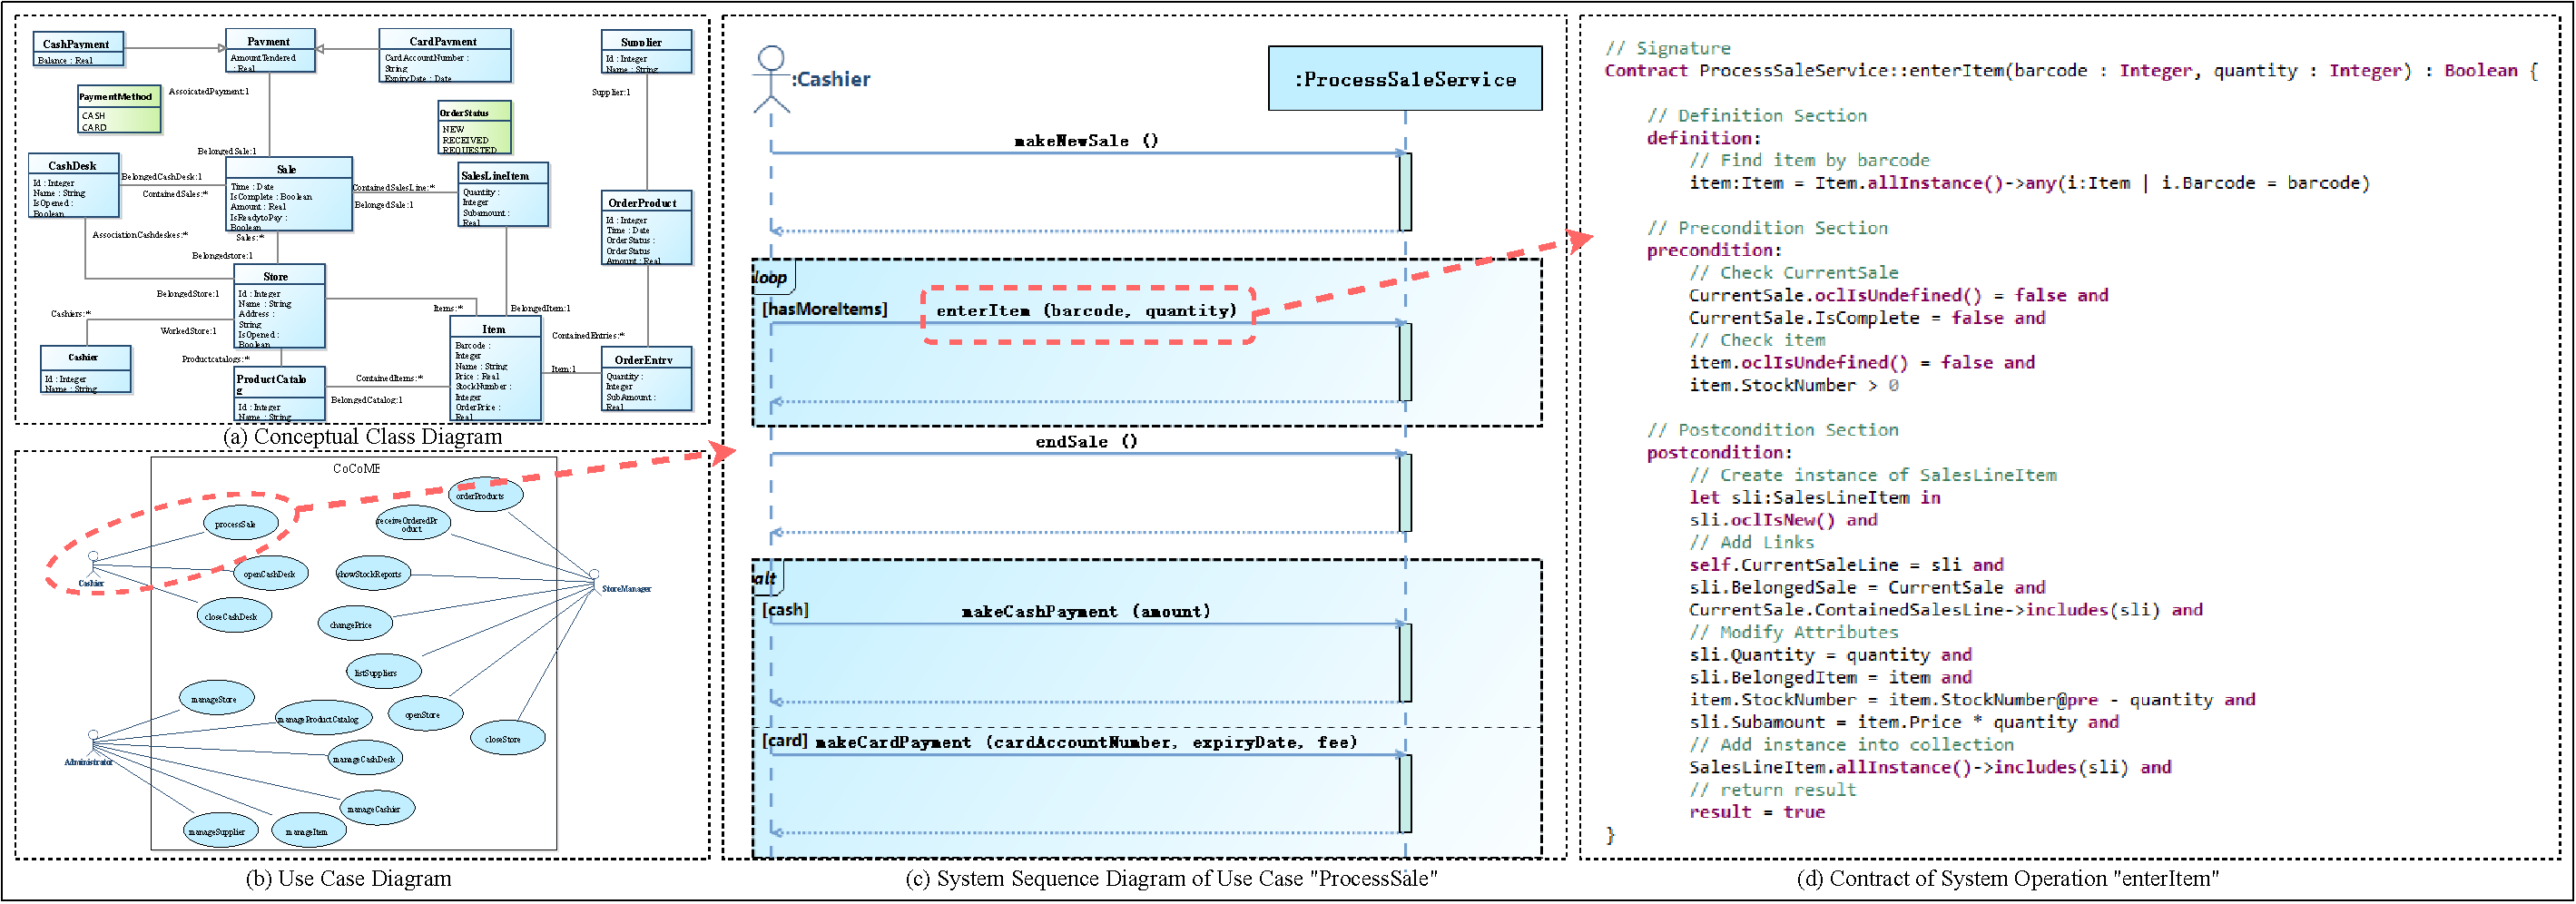
\includegraphics[width=\textwidth]{images/requirementsmodel.pdf}
  \caption{Requirements Model}\label{rm}
\end{figure*}
\subsection{\textcolor{red}{Requirements and Design Models}}

\textcolor{red}{The requirements model adopted in our approach consists of four components, as illustrated in Figure~\ref{rm}:}
\begin{itemize}
    \item \textcolor{red}{\textbf{Use Case Diagram:} Describes interactions between actors and the system to capture user goals.}
    \item \textcolor{red}{\textbf{Conceptual Class Diagram:} Depicts domain concepts and their relationships, without specifying operations or implementation details.}
    \item \textcolor{red}{\textbf{System Sequence Diagrams:} Shows the sequence of system operations for each use case, treating the system as a black box.}
    \item \textcolor{red}{\textbf{Contracts of System Operations:} Formally specifies pre- and post-conditions of each system operation using OCL\cite{LWFM1,RM1,RM2,RM3,YangTR}.}
\end{itemize}

\textcolor{red}{The design model generated by our approach comprises a class diagram and sequence diagrams. The class diagram defines the static structure, including classes, attributes, operations, and relationships such as aggregation, composition, and inheritance. Sequence diagrams capture the dynamic interactions among objects by detailing the messages exchanged to realize each system operation. The key distinction from the requirements model is that design-level class diagrams specify operations and encapsulation strategies, while sequence diagrams reveal internal object interactions rather than treating the system as a black box. Examples of the generated design model are shown in Figures~\ref{cde}, \ref{cds}, and~\ref{sd}.}

\begin{figure*}[!htb]
  \centering
  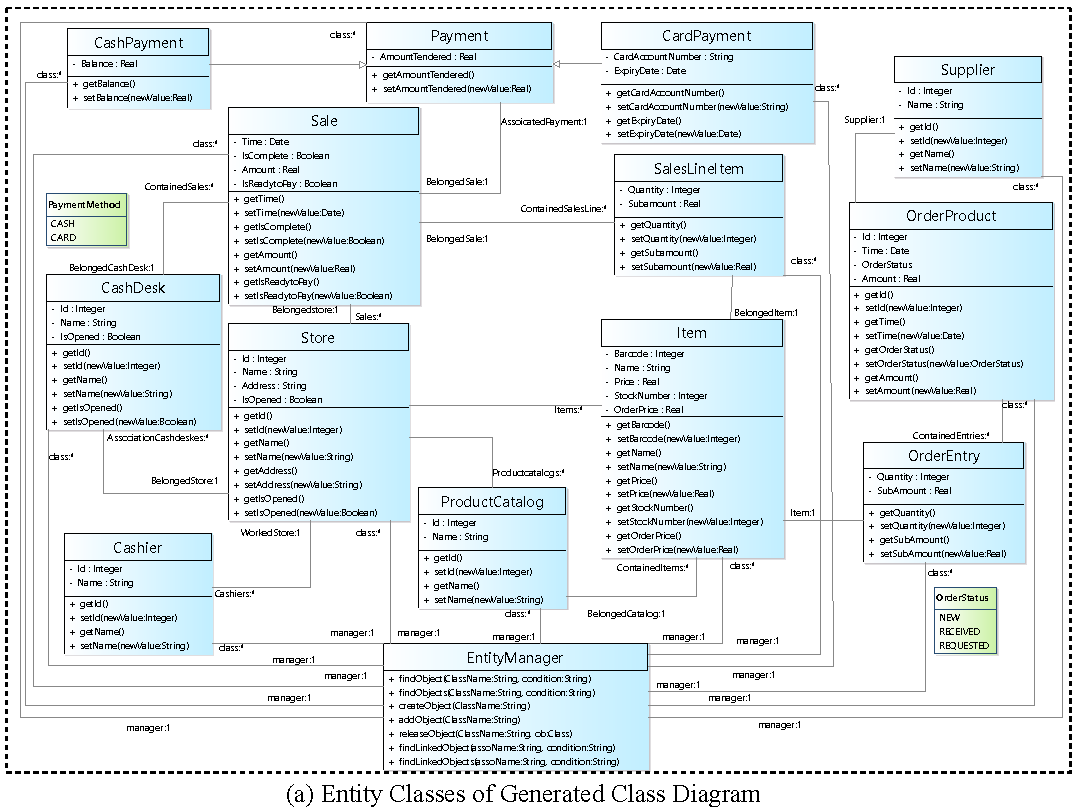
\includegraphics[width=1\textwidth]{images/ClassDiagram-Entity.pdf}
  \caption{Generated Class Diagram Entity Part}\label{cde}
\end{figure*} 

\begin{figure*}[!htb]
  \centering
  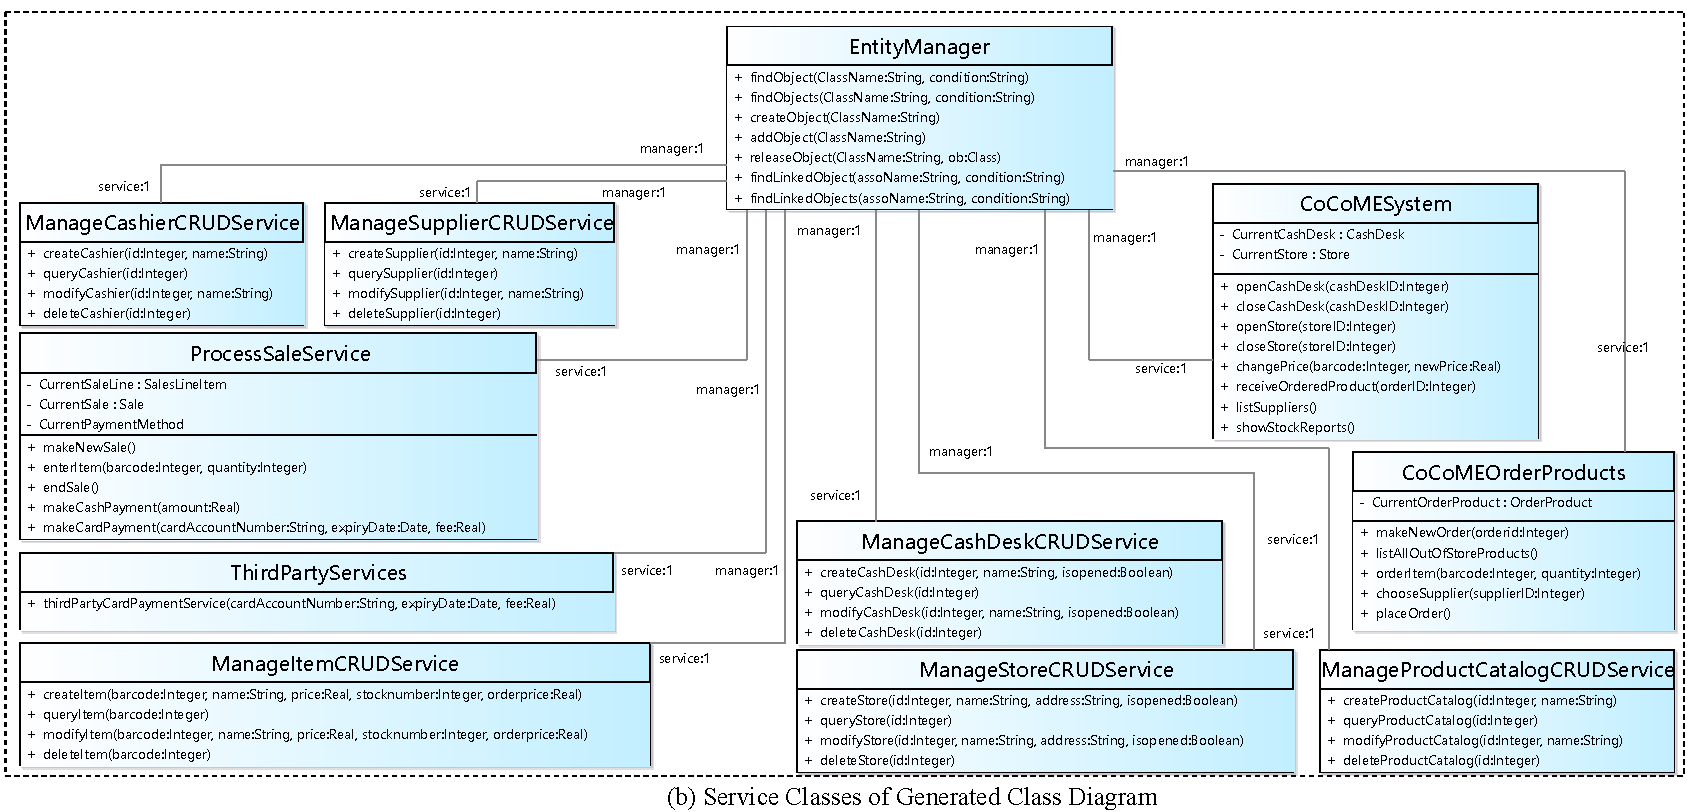
\includegraphics[width=1\textwidth]{images/ClassDiagram-service.pdf}
  \caption{Generated Class Diagram Service Part}\label{cds}
\end{figure*} 

\begin{figure*}[!htb]
    \centering
    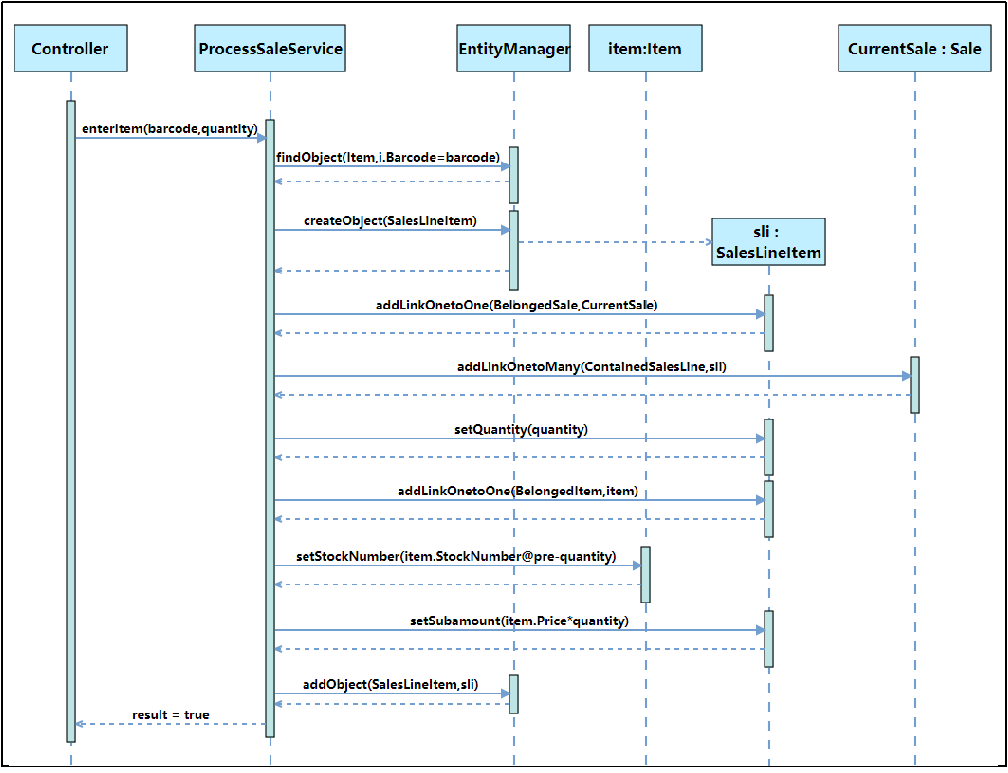
\includegraphics[width=.8\textwidth]{images/SequenceDiagram.pdf}
    \caption{Generated Sequence Diagram for System Operation ``enterItem"}
    \label{sd}
\end{figure*}

\subsection{Anemic Domain Model}
\textcolor{red}{The anemic domain model~\cite{DDD} structures the system into three layers: Domain (entities and value objects with data and basic operations), Service (business logic), and Repositories (data persistence and querying). Unlike rich domain models where entities encapsulate both data and business logic, the anemic model places business logic in the Service layer, making entities thin data containers. Despite being considered a design anti-pattern, the anemic model is widely adopted in practice, particularly in web applications where business logic primarily involves CRUD operations, and is supported by mainstream frameworks such as Java EE and Spring. Our approach targets this prevalent architectural style.}

\subsection{Rule-based Agents and LLMs-based Agents}
%软件智能体和多智能体系统从上世纪80年代开始就得到了相当多的研究。智能体作为一个自治的系统，能够和其他智能体交互以满足其设计目标\cite{}。
Software agents and multi-agent systems have received considerable research attention since the 1980s\cite{AgentOrientedSoftwareEngineering}. An agent, as an autonomous system, is capable of interacting with other agents to fulfill its designed objectives. Multi-Agent Systems (MAS) consist of multiple autonomous entities, or agents, that interact within a shared environment to achieve individual or collective goals. In the research of agent-oriented software engineering, the primary focus is on how to utilize agents as fundamental building modules for designing and developing complex systems, with an emphasis on modularity, reusability, and software architecture. The agents therein typically operate based on predefined rules or logical reasoning, and their interactions mainly base on rule and deterministic protocols or algorithms. We refer to this kind of agent as Rule-based Agents.

Large Language Models are a class of deep learning models designed to understand and generate human-like text. LLMs leverage massive datasets and billions of parameters to achieve remarkable language comprehension and generation capabilities. Due to the rapid development of LLMs, LLMs-based agents have attracted significant attention. LLMs-based agents take LLMs as the core. Through reinforcement learning and function-calling techniques, such agents can automate complex tasks via the ``perceive-decide-act" process.

\section{Approach}
This section describes our method for transforming requirement models into design models (including a class diagram and sequence diagrams), assessing design quality during the design phase, and offering straightforward refactoring recommendations.
\subsection{Overview}

\begin{figure*}[!htb]
    \centering
    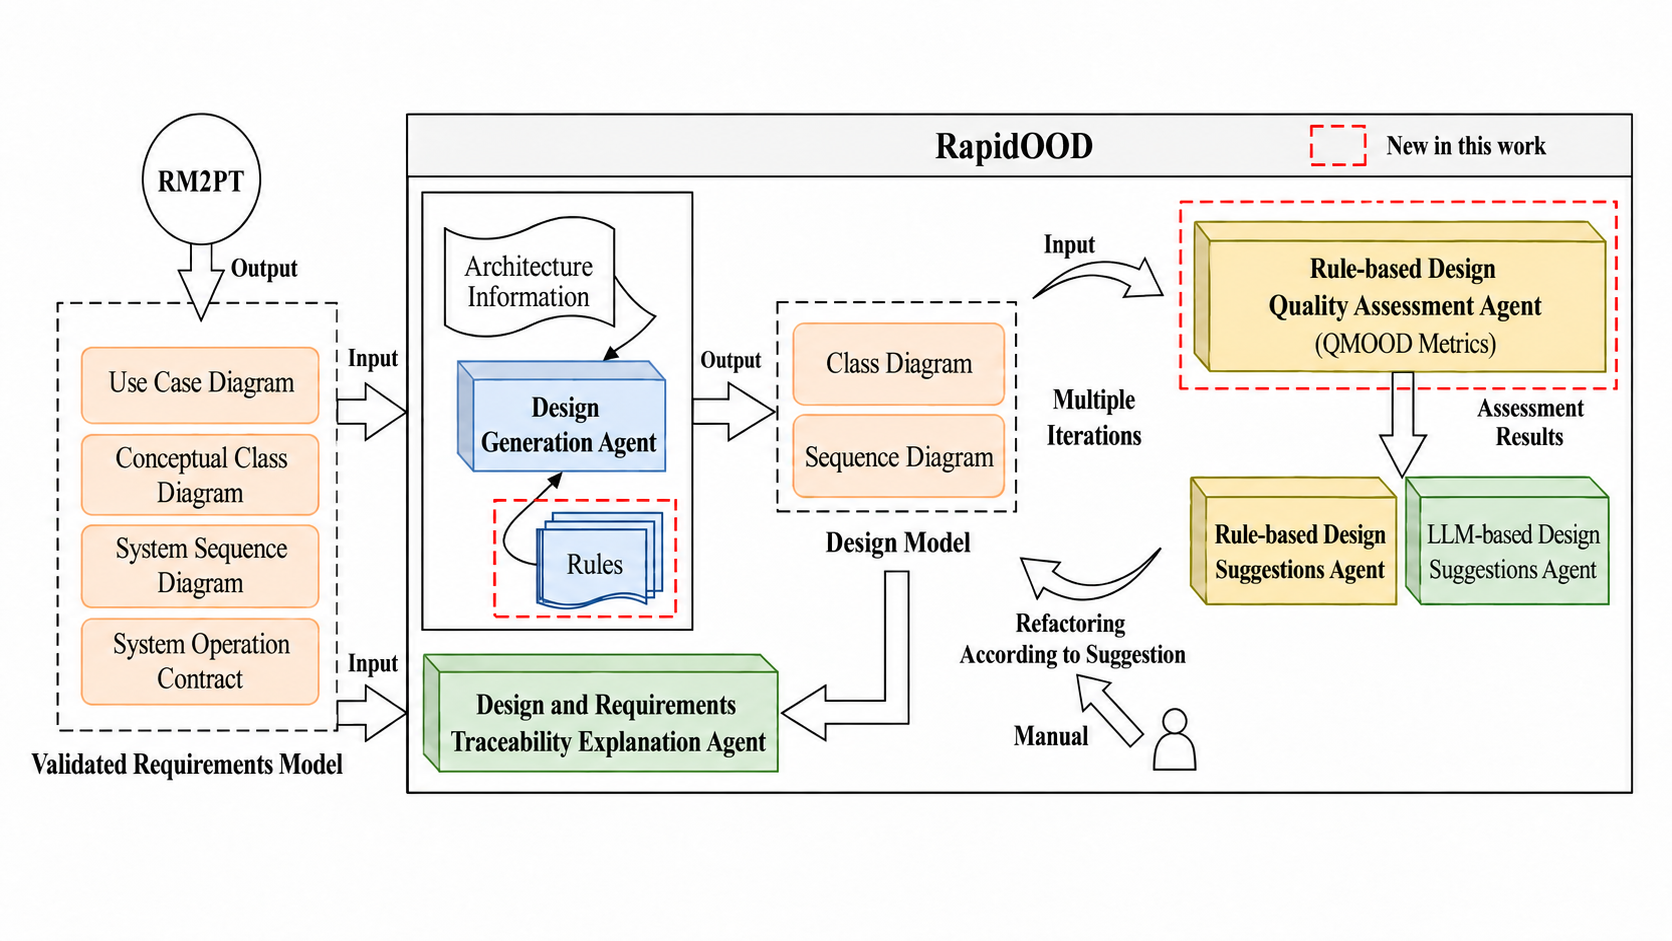
\includegraphics[width=1\textwidth]{images/ChatGPT Image 2026年9月22日 09_47_57.png}
    \caption{Overview of RapidOOD. Red dashed boxes indicate capabilities newly introduced in this work compared with RM2DM.}
\label{Overview}
\end{figure*}

Our approach takes validated requirements models as input. Auto-prototyping work, such as RM2PT, assists in swiftly attaining a validated requirements model by automatically producing prototypes from requirement models, thereby facilitating incremental and agile requirements validation. We propose a set of rules and algorithms to generate the design models composed of a class diagram and a set of sequence diagrams. Based on the initial design models generated, we employ QMOOD, a hierarchical model for evaluating the quality of object-oriented designs, to assess the design quality. The results of the quality assessment metrics and the simple refactoring suggestions we propose are fed back to the users. Users can then manually iterate on the design based on this feedback, thereby swiftly achieving a relatively higher quality design.

In this paper, the agents are not solely centered around LLMs, instead, the framework incorporates a hybrid approach where agents are built upon both LLM-driven capabilities and traditional model-driven methods. While LLM-based agents excel in tasks requiring natural language understanding, reasoning, and adaptability, the model-driven agents leverage predefined rules, domain-specific models, and structured decision-making processes to handle tasks with deterministic logic or stringent performance requirements. This duality allows the system to balance the flexibility of LLMs with the reliability and efficiency of traditional approaches, creating a more robust and versatile multi-agent framework.

In RapidOOD, we designed the Design Generation Agent, Design Quality Assessment Agent, and rule-based Design Suggestions Agent that provides simple recommendations using a model-driven, rule-based approach. The model-driven approach generates the initial design model from the requirements model, ensuring excellent traceability and the scale of the initial design. (As can be seen in the subsequent experimental section, the design models generated solely by LLMs are limited in scale and often lack essential relationships or operations.) For the quality assessment of the design, a quantitative method based on QMOOD Metrics was adopted. By statistically analyzing the model elements of the design model, high-level quality attribute metrics of the design model were obtained, such as reusability. For low quality attributes, rule-based design refactoring suggestions were provided. For example, parts with high coupling in the design model were highlighted and suggestions for refactoring were given.

We designed the LLM-Based Design Suggestions Agent and the Traceability Explanation Agent. The aim is to utilize the knowledge-emergence ability of LLMs to provide expert-level design refactoring suggestions and to offer easily understandable explanations for the traceability between the design and the requirements.

\subsection{Design Model Generation Agent}
\subsubsection{Transformation Rules of Class Diagram Generation}
Three transformation rules are proposed to automatically generate a class diagram from the requirement model .
\paragraph{Preserve the Classes and Relationships}
The first rule is to preserve the relationships between classes and classes in the conceptual class diagram and add GET/SET methods corresponding to the class attributes. This design is based on the fact that the relationships between classes and classes in the conceptual class diagram in the requirement model are naturally consistent with the actual situation, and this part should remain the same; otherwise, relationship errors or missing relationships will occur.
\paragraph{Generate Service Class}
The second rule is to encapsulate all use case-related system operations into a new Service class based on the use case diagram (including use cases) and the system sequence diagram (including system operations related to use cases). For a case, according to the information in the use case diagram and the system sequence diagram, a new class is extracted, which contains the class name, attributes, operations, and other information. It extracts class names from use case diagrams and attributes and operations from system sequence diagrams and system operation contracts.

The classes extracted by this rule will serve as the content of the Service layer and can be used to provide services to the outside world. Service will act as the initiator of the system operation, and then the various classes within the system will work together to complete the various system operations.
\paragraph{Generate EntityManager Class}
The third rule involves the creation of a new EntityManager class, which serves as the central hub for all other classes. It is responsible for adding, deleting, modifying, and querying objects, and thus should have primitive operations related to these tasks.
The operations owned by EnitityManager are derived by summarizing the OCL statements in the system operation contract. 10 types of OCL expressions associated with EnitityManager and 7 primitive operations are needed.
\begin{gather*}
   \textit{$E_1: obs: Set (ClassName) = ClassName.allInstances()$}\\
   \textit{$E_2: obs: Set (ClassName) = ClassName.allInstances()$}\\
   \textit{$-> select (o | conditions(o))$}
\end{gather*}

The meaning of statement 1 is to find instances of all ClassName classes in the system, and the meaning of statement 2 is to find instances of conditional conditions of all ClassName classes in the system. To complete the behavior described by the two OCL statements, the class EntityManager requires the operation findObjects().
\begin{gather*}
    E_3: ob: ClassName = ClassName.allInstances()\\
    -> any (o | conditions(o))
\end{gather*}

The meaning of statement 3 is to find an instance of a conditional condition of any ClassName class in the system. Therefore, the class EnitityManager requires a findObject() operation.
\begin{gather*}
E_4: o: ClassName = ob.assoName\\
E_5: o: ClassName = ob.assoName \\
-> any (o | conditions(o))    
\end{gather*}

Statement 4 means to find a single instance of a class in the system that has an assoName relationship with an ob class, and statement 5 means to find any instance of a conditional condition of a class that has an assoName relationship with an OB class in the system. Both statements find a single object based on the association relationship, so the EnitityManager needs an operation findLinkedObject ().
\begin{gather*}
   E_6: obs: Set (ClassName) = ob.assoName\\
   E_7: obs: Set (ClassName) = ob.assoName\\
   -> select (o | conditions(o)) 
\end{gather*}

The meaning of statement 6 is to find a collection of instances of a class in the system that has an assoName relationship with an ob class, and the meaning of statement 7 is to find a collection of instances of a conditional class in the system that has an assoName relationship with an ob class, so the EnitityManager needs to be able to find a collection of objects based on the association relationship and needs to operate findLinkedObjects ().
\begin{gather*}
   E_8: let ob: ClassName in ob.oclIsNew() 
\end{gather*}

The meaning of statement 8 is to define an object OB for a ClassName, so the EnitityManager needs to be able to create instances of a particular class and needs to have an operation createObject ().
\begin{gather*}
  E_9: ClassName.allInstances() -> includes (ob)  
\end{gather*}

Statement 9 appears in the Postcondition section of the system operation contract, indicating that the OB object needs to be guaranteed to be included in the instance of ClassName after the system operation is executed, so EnitityManager needs to add the OB object to the list of instances of ClassName class, and the addObject () operation is required.
\begin{gather*}
  E_{10}: ClassName.allInstances() -> excludes(ob)  
\end{gather*}

Statement 10 appears in the Postcondition section of the system operation contract, indicating that you need to ensure that the ClassName instance after the system operation is executed does not contain an ob object, so EnitityManager needs to remove the OB object from the list of ClassName instances, and you need an operation releaseObject().

\subsubsection{Transformation Rules of Sequence Diagram Generation}
RapidOOD uses sequence diagrams to describe the collaboration of objects within the system. The main content of the sequence diagram is the messages passed between objects. Based on the anemic domain model, there is a controller in the system. The controller sends the invocation messages of system operations to the corresponding service class. The service class sends messages to the related objects inside the system, and the objects collaborate to complete the system operations and return.
The primary challenge lies in the generation of messages between objects. Of the three components of the system operation contract, the OCL expressions in the precondition part define the system's required state before executing the operation. As these preconditions do not involve interactions between class instances, they are not converted into messages. The definition and post-condition of the system operation contract, on the other hand, describe the system's dynamic behavior. The OCL expressions in these sections can be transformed into messages in sequence diagrams. To facilitate this transformation, a set of 17 transformation rules has been established. Transformation rules are presented in this form:
% $$
% Rule : \frac{OCL Expression}{Message Label, Sender, Receiver}
% $$
\[
\begin{array}{l}
    \textit{Rule}: \frac{\textit{OCL Expression}}{\textit{Message Label, Sender, Receiver}}
\end{array}
\]

The transformation rule contains two parts: the above is an OCL expression in the contracts, and the bottom part is the generated message and the message's sender and receiver.

\[
\begin{array}{l}
    \textit{R1}: \frac{\textit{obs: Set (ClassName)= ClassName.allInstances()}}{\textit{findObjects (ClassName),Service,EnitityManager}}
\end{array}
\]

\[
\begin{array}{l}
    \textit{R2}: \frac{\textit{obs: Set (ClassName) = ClassName.allInstances() → select (o $|$ conditions(o))}}{\textit{findObjects (ClassName,conditions (o)),Service,EntityManageer}}
\end{array}
\]

\[
\begin{array}{l}
    \textit{R3}: \frac{\textit{ob: ClassName = ClassName.allInstances() → any (o $|$ conditions(o))}}{\textit{findObject (ClassName,conditions (o)),Service,EntityManageer}}
\end{array}
\]

\[
\begin{array}{l}
    \textit{R4}: \frac{\textit{o: ClassName = ob.assoName}}{\textit{findLinkedObject (ob,assoName),Service,EntityManageer}}
\end{array}
\]

\[
\begin{array}{l}
    \textit{R5}: \frac{\textit{o: ClassName = ob.assoName -> any (o | conditions(o))}}{\textit{findLinkedObject (ob,assoName,conditions(o)),Service,EntityManageer}}
\end{array}
\]

\[
\begin{array}{l}
    \textit{R6}: \frac{\textit{obs: Set (ClassName) = ob.assoName}}{\textit{findLinkedObjects (ob,assoName),Service,EntityManageer}}
\end{array}
\]

\[
\begin{array}{l}
    \textit{R7}: \frac{\textit{obs: Set (ClassName) = ob.assoName -> select (o | conditions(o))}}{\textit{findLinkedObjects (ob,assoName,conditions(o)),Service,EntityManageer}}
\end{array}
\]

Rules 1 to 7 are the conversion rules from the definition part of the OCL statement to the message. The meaning of this part of the statement has been introduced above. According to this part of the conversion rules, the sending end of the message is Service, and the receiving end is EntityManager.

\[
\begin{array}{l}
    \textit{R8}: \frac{\textit{let ob: ClassName in ob.oclIsNew()}}{\textit{createObject (ClassName),EntityManageer,ob}}
\end{array}
\]

The meaning of statement 8 is to generate an instance ob of the ClassName class. The operation of creating an object is initiated by the Service and completed by the EntityManager to generate an object ob. There are actually two request messages in this process. One is that the Service sends a message to the EntityManager to request the creation of an instance; the other is the creation message of the object ob created by the EntityManager.

\[
\begin{array}{l}
    \textit{R9}: \frac{\textit{ClassName.allInstances() -> includes (ob)}}{\textit{addObject (ClassName,ob),Service,EntityManageer}}
\end{array}
\]

\[
\begin{array}{l}
    \textit{R10}: \frac{\textit{ClassName.allInstances() -> excludes(ob)}}{\textit{releaseObject (ClassName,ob),Service,EntityManageer}}
\end{array}
\]

Statement 9 and statement 10 are the OCL statements of the postcondition part, and the related class is also EnitityManager, which has been introduced in the previous article. For the messages obtained according to rules 9 and 10, the sending end is Service, and the receiving end is EntityManager.
\[
\begin{array}{l}
    \textit{R11}: \frac{\textit{ob.assoName -> includes(addOb)}}{\textit{addLinkOnetoMany (assoName,addOb),Service,ob}}
\end{array}
\]

The meaning of statement 11 is to add the addOb object to the list of objects pointed to by the assoName relation of ob, corresponding to the atomic operation addLinkOnetoMany(), which is executed by the object ob.

\[
\begin{array}{l}
    \textit{R12}: \frac{\textit{ob.assoName ->excludes(removeOb)}}{\textit{removeLinkOnetoMany (assoName,removeOb),Service,EntityManageer}}
\end{array}
\]

The meaning of statement 12 is to remove the removeOb object from the list of objects pointed to by the assoName relation of ob, and the corresponding atomic operation is removeLinkOnetoOne(), which is executed by the object ob.

\[
\begin{array}{l}
    \textit{R13}: \frac{\textit{ob.assoName = addOb}}{\textit{addLinkOnetoOne (assoName,addOb),Service,ob}}
\end{array}
\]

The meaning of statement 13 is to change the object pointed to by the assoName relation of ob to addOb, and the corresponding atomic operation is addLinkOnetoOne(), which is executed by the object ob.

\[
\begin{array}{l}
    \textit{R14}: \frac{\textit{ob.assoName = null}}{\textit{removeLinkOnetoOne (assoName),Service,ob}}
\end{array}
\]

The meaning of statement 14 is to change the object pointed to by the assoName relation of ob to null, i.e., it does not point to any object, and the corresponding atomic operation is removeLinkOnetoOne(), which is executed by the object ob.

\[
\begin{array}{l}
    \textit{R15}: \frac{\textit{ob.attriName = mathExp}}{\textit{setAttriName (mathExp),Service,ob}}
\end{array}
\]

The meaning of statement 15 is to change the value of the attriName attribute of ob to the value represented by mathExp, and the corresponding atomic operation is setAttribute(), which is executed by the object ob.

\[
\begin{array}{l}
    \textit{R16}: \frac{\textit{result = var}}{\textit{return (var),Service,Controller}}
\end{array}
\]

The meaning of statement 16 is to return the result of the system operation. 

\[
\begin{array}{l}
    \textit{R17}: \frac{\textit{ThirdPartyService.opName(vars)}}{\textit{opName (vars),Service,ThirdPartyService}}
\end{array}
\]

The meaning of statement 17 is to call a method of a third-party service.
For each OCL expression in the system operation contract, apply rules 1-7 if it belongs to the definition part of the contract and rules 8-17 if it belongs to the post-condition part. Determine the rules for the OCL expression based on its syntactic structure. Apply the rules to extract the label, the sending object and receiving object of the message from the OCL expression.

\begin{algorithm}
\caption{Sequence Diagram Messages Generation}
\label{algA}
    \begin{algorithmic}[1]
        \REQUIRE System Operation Contract
        \ENSURE Sequence Diagram Messages
        \FOR{each $OCLExpression \in Contract$}
            \IF{$OCLExpression \in \text{definition}$}
                \STATE applyRule($1-7$)
            \ELSIF{$OCLExpression \in \text{postcondition}$}
                \STATE applyRule($8-17$)
            \ENDIF
        \ENDFOR
        \STATE \textbf{procedure} applyRule($ruleOrder$)
        \STATE \quad setMessageLabel()
        \STATE \quad setMessageSender()
        \STATE \quad setMessageReceiver()
    \end{algorithmic}
\end{algorithm}
% \begin{algorithm}
% \caption{Sequence Diagram Messages Generation}
% \label{algA}
%     \begin{algorithmic}
%         \REQUIRE System Operation Contract
%         \ENSURE Sequence Diagram Messages
%         \FOR{each $ OCLExpression \  \textbf{in} \  Contract$}
%             \IF{$ OCLExpression \in definition $}
%                 \STATE applyRule($1-7$)
%             \ELSIF{$ OCLExpression \in postcondition $}
%                 \STATE applyRule($8-17$)
%             \ENDIF
%         \ENDFOR
%         \renewcommand{\algorithmicrequire}{\textbf{applyRule}}
%         \REQUIRE{($ruleOrder$)} 
%             \STATE setMessageLabel()
%             \STATE setMessageSender()
%             \STATE setMessageReceiver()
%     \end{algorithmic}
% \end{algorithm}


Algorithm \ref{algA} shows how to apply the rules to generate messages from system operation contracts. For each OCL expression in the system operation contract, apply rules 1-7 if it belongs to the definition part of the contract and rules 8-17 if it belongs to the post-condition part. Determine the rules for the OCL expression based on its syntactic structure. Apply the rules to extract the label, the sending object and receiving object of the message from the OCL expression.

Algorithm \ref{algB} describes how to order OCL statements to ensure that they are executable. It involves constructing a dependency graph and performing topological sorting to ensure that all dependencies are respected. The algorithm details are as follows.

\textbf{Initialize the Dependency Graph}: Create an empty directed graph $G = (V, E)$, where $V$ represents the set of nodes (OCL statements) and $E$ represents the set of directed edges (dependencies between statements).

\textbf{Add Nodes to the Graph}: For each OCL statement $s_i \in S$ (where $S$ is the set of OCL statements), add $s_i$ as a node in $V$.

\textbf{Add Edges to the Graph}: For each OCL statement $s_i \in S$, identify its dependencies. For each dependency $s_j$ of $s_i$, add a directed edge $(s_j, s_i)$ to $E$. This indicates that $s_i$ depends on $s_j$.

\textbf{Topological Sorting Initialization}: Initialize an empty list $L$ to store the sorted OCL statements. Initialize an empty set $S$ to store all nodes with no incoming edges.

\textbf{Identify Nodes with No Incoming Edges}: For each node $v \in V$, if $v$ has no incoming edges, add $v$ to $S$.

\textbf{Topological Sorting Process}: While $S$ is not empty:
- Remove a node $n$ from $S$.
- Add $n$ to $L$.
- For each node $m$ such that $(n, m) \in E$:
  - Remove edge $(n, m)$ from $E$.
  - If $m$ has no other incoming edges, add $m$ to $S$.

\textbf{Cycle Detection}: If there are any remaining edges in $E$, this indicates that the graph $G$ contains at least one cycle, and a topological sorting is not possible. In this case, report an error.

\textbf{Return the Sorted List}: Return the list $L$ as the topologically sorted order of OCL statements.
% \begin{enumerate}
%     \item \textbf{Initialize the Dependency Graph}:
%     \begin{itemize}
%         \item Create an empty directed graph $G = (V, E)$, where $V$ represents the set of nodes (OCL statements) and $E$ represents the set of directed edges (dependencies between statements).
%     \end{itemize}
    
%     \item \textbf{Add Nodes to the Graph}:
%     \begin{itemize}
%         \item For each OCL statement $s_i \in S$ (where $S$ is the set of OCL statements), add $s_i$ as a node in $V$.
%     \end{itemize}
    
%     \item \textbf{Add Edges to the Graph}:
%     \begin{itemize}
%         \item For each OCL statement $s_i \in S$, identify its dependencies. For each dependency $s_j$ of $s_i$, add a directed edge $(s_j, s_i)$ to $E$. This indicates that $s_i$ depends on $s_j$.
%     \end{itemize}
    
%     \item \textbf{Topological Sorting Initialization}:
%     \begin{itemize}
%         \item Initialize an empty list $L$ to store the sorted OCL statements.
%         \item Initialize an empty set $S$ to store all nodes with no incoming edges.
%     \end{itemize}
    
%     \item \textbf{Identify Nodes with No Incoming Edges}:
%     \begin{itemize}
%         \item For each node $v \in V$, if $v$ has no incoming edges, add $v$ to $S$.
%     \end{itemize}
    
%     \item \textbf{Topological Sorting Process}:
%     \begin{itemize}
%         \item While $S$ is not empty:
%         \begin{enumerate}
%             \item Remove a node $n$ from $S$.
%             \item Add $n$ to $L$.
%             \item For each node $m$ such that $(n, m) \in E$:
%             \begin{itemize}
%                 \item Remove edge $(n, m)$ from $E$.
%                 \item If $m$ has no other incoming edges, add $m$ to $S$.
%             \end{itemize}
%         \end{enumerate}
%     \end{itemize}
    
%     \item \textbf{Cycle Detection}:
%     \begin{itemize}
%         \item If there are any remaining edges in $E$, this indicates that the graph $G$ contains at least one cycle, and a topological sorting is not possible. In this case, report an error.
%     \end{itemize}
    
%     \item \textbf{Return the Sorted List}:
%     \begin{itemize}
%         \item Return the list $L$ as the topologically sorted order of OCL statements.
%     \end{itemize}
% \end{enumerate}

\begin{algorithm}[H]
\caption{OCL Statement Execution Order Sorting}
\label{algB}
\begin{algorithmic}[1]
\REQUIRE A set of OCL statements $S = \{s_1, s_2, \ldots, s_n\}$ with dependencies
\ENSURE A topologically sorted list of OCL statements
\STATE Initialize an empty dependency graph $G = (V, E)$
\FOR{each $s_i \in S$}
    \STATE Add $s_i$ as a node in $V$
\ENDFOR
\FOR{each $s_i \in S$}
    \FOR{each $s_j \in \text{dependencies}(s_i)$}
        \STATE Add a directed edge $(s_j, s_i)$ to $E$
    \ENDFOR
\ENDFOR
\STATE Initialize an empty list $L$ to store the sorted OCL statements
\STATE Initialize an empty queue $Q$ to store all nodes with no incoming edges
\FOR{each $v \in V$}
    \IF{v has no incoming edges}
        \STATE Add $v$ to $Q$
    \ENDIF
\ENDFOR
\WHILE{$Q$ is not empty}
    \STATE Remove a node $n$ from $Q$
    \STATE Add $n$ to $L$
    \FOR{each node $m$ such that $(n, m) \in E$}
        \STATE Remove edge $(n, m)$ from $E$
        \IF{m has no other incoming edges}
            \STATE Add $m$ to $Q$
        \ENDIF
    \ENDFOR
\ENDWHILE
\IF{any edges remain in $E$}
    \STATE \textbf{error}: Graph $G$ has at least one cycle
\ENDIF
\RETURN $L$
\end{algorithmic}
\end{algorithm}


\subsection{Quality Assessment and Refactoring Recommendations of Design Model}
% We evaluate design quality using QMOOD, a hierarchical model for object-oriented design quality assessment. In the QMOOD method, the high-level quality attribute indicators are calculated from the low-level element statistical indicators. In the original approach, this evaluation is based on code. However, we noticed that many of these underlying metrics were available early in the design phase of the project, empowering designers to make proactive decisions. For example, QMOOD uses the number of classes to represent the size of the design, which is determined when the design is completed. Another example is the number of levels. In a hierarchical architecture, the value of the number of levels is fixed and can also be obtained at design time.

% Based on the evaluation results of quality attributes, we provide simple rule-based design optimization recommendations to designers. Since the calculation of high-level quality attribute indicators is based on the statistical number of underlying elements, we can identify the design elements that most impact a particular quality attribute indicator. We decided to set the granularity of design elements to classes, and when a class was found to have the most significant negative impact on specific quality attribute metrics, we highlighted it and suggested that designers make optimizations.

We evaluated design quality using QMOOD, a hierarchical model to evaluate object-oriented design quality. In the QMOOD method, the high-level quality attribute indicators are calculated from the low-level element statistical indicators. Traditionally, this quality assessment is based on code. However, we noticed that many of these underlying metrics were available early in the design phase of the project, empowering designers to make proactive decisions. For example, QMOOD uses the number of classes to represent the size of the design, which is determined when the design is completed. Another example is the number of levels in a hierarchical architecture, whose value is fixed and can also be obtained at design time.
\subsubsection{Rule-based Design refactoring Agent}
Based on the results of the quality attributes assessment, we provide simple rule-based design refactoring recommendations to designers. Since the calculation of high-level quality attribute indicators is based on the statistical number of underlying elements, we can identify the design elements that most impact a particular quality attribute indicator. We decided to set the granularity of design elements to classes, and when a class was found to have the most significant negative impact on specific quality attribute metrics, we highlighted it and suggested that designers make refactorings.

\begin{itemize}
    \item Design size: Consider the case where the number of classes exceeds a threshold that indicates complexity. This metric is available early in the design phase. If the number of classes is too high, we recommend strategies such as refactoring into smaller modules or applying design patterns like the Factory pattern to manage complexity.
    \item Hierarchy: In a hierarchical architecture, if the number of levels is too deep, indicating a potential for maintenance issues, we suggest flattening the structure by merging similar classes or using composition over inheritance where appropriate.
    \item Coupling: When the coupling between classes is too high, indicating a lack of modularity, we recommend introducing interfaces or applying the Dependency Injection pattern to decouple components.
    \item Cohesion: If the cohesion within a class is low, suggesting that the class has multiple responsibilities, we advise splitting the class into smaller, more focused classes or applying the Single Responsibility Principle.
    \item Polymorphism: If there is a high degree of polymorphism, indicating a complex inheritance hierarchy, we recommend simplifying the inheritance structure by reducing the depth of the hierarchy or employing composition instead of inheritance.
\end{itemize}

For example, in the generated class diagram shown in Figure \ref{cde}, we can see that the EntityManager class has the most significant number of directly related classes, which has the highest degree of coupling according to the metric calculation, thus suggesting a design refactoring for it: ``EntityManager has high Direct Class Coupling, please pay attention to proper class responsibility division". Considering the refactoring of EntityManager, in this design, EntityManager is mainly responsible for receiving the requests of the service layer and modifying the attributes and association relations of the related classes in the entity layer. The EntityManager can be split into multiple repositories, each responsible for modifying a class. This reduces the degree of coupling between classes, and the responsibility of each class is more single, in line with the single responsibility principle. We can see that this modification has changed some of the low-level design metrics and affected the high-level design quality. Understandability decreases because multiple managers are more complex than a single Manager in terms of design structure. However, splitting it into various managers makes for better readability. Functionality goes up because multiple Managers bring access to multiple common interfaces. Less coupling between classes also leads to better reusability, flexibility, and extensibility. This example illustrates the effectiveness of the refactoring method according to quality metrics.

\begin{figure*}[!htb]
  \centering
  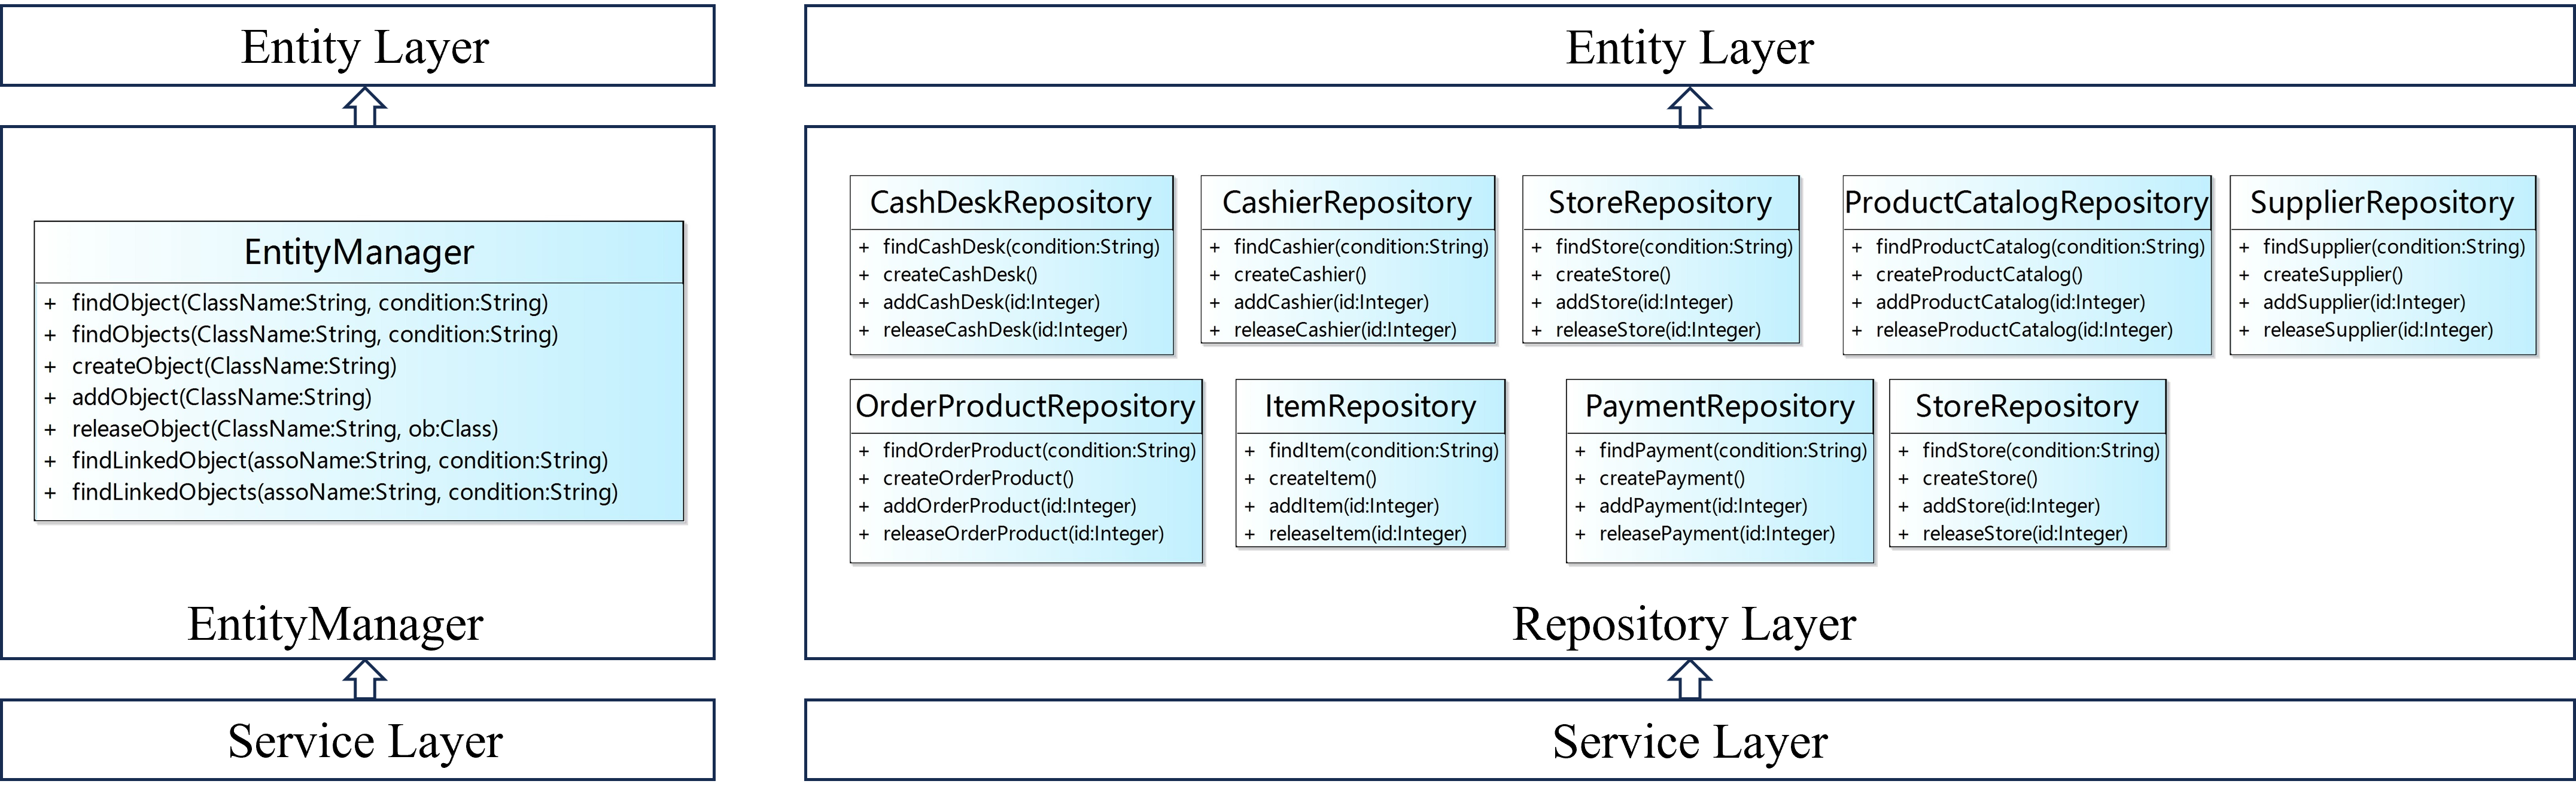
\includegraphics[width=1\textwidth]{images/ClassDiagramWithRepo.png}
  \caption{Optimized Class Diagram}\label{ocd}
\end{figure*}

\begin{table*}[]
\caption{Comparison of Design Quality Indicators Before and After Modification}
  \label{Design Metric Results}
  \centering
  \resizebox{\linewidth}{!}{
\begin{tabular}{@{}llllllllllll@{}}
\toprule
Metric       & DSC                            & NOH    & ANA                           & DAM    & DCC                           & CAM    & MOA    & MFA    & NOP    & CIS                             & NOM                             \\ \midrule
Before       & 24.0000                        & 3.0000 & 0.0833                        & 1.0000 & 2.7917                        & 1.0000 & 5.0000 & 0.4500 & 1.0000 & 144.0000                        & 144.0000                        \\
After        & {\color[HTML]{C00000} 32.0000} & 3.0000 & {\color[HTML]{548235} 0.0625} & 1.0000 & {\color[HTML]{548235} 2.0625} & 1.0000 & 5.0000 & 0.4500 & 1.0000 & {\color[HTML]{C00000} 173.0000} & {\color[HTML]{C00000} 173.0000} \\
After/Before & 1.3333                         & 1.0000 & 0.7503                        & 1.0000 & 0.7388                        & 1.0000 & 1.0000 & 1.0000 & 1.0000 & 1.2014                          & 1.2014                          \\ \bottomrule
\end{tabular}}
\end{table*}

\begin{table*}[]
\caption{Comparison of Design Quality Before and After Modification}
  \label{Design Quality Results}
  \centering
  \resizebox{\linewidth}{!}{
\begin{tabular}{@{}lllllll@{}}
\toprule
Metric & Resuability                   & Flexibility                   & Understandability              & Functionality                 & Extendibility                 & Effectiveness                 \\ \midrule
Before & 1.0000                        & 1.0000                        & -0.9900                        & 1.0000                        & 1.0000                        & 1.0000                        \\
After  & {\color[HTML]{C00000} 1.3327} & {\color[HTML]{C00000} 1.0653} & {\color[HTML]{548235} -0.9979} & {\color[HTML]{C00000} 1.1176} & {\color[HTML]{C00000} 1.0058} & {\color[HTML]{548235} 0.9501} \\ \bottomrule
\end{tabular}}
\end{table*}

\subsubsection{LLM-based Design refactoring Agent}
%TODO：可能需要修改表述
The rapid development of Large Language Models (LLMs), such as GPT, BERT, and their successors, has revolutionized various domains by providing unprecedented capabilities in natural language understanding and generation. These models are not only reshaping industries like customer support, content creation, and data analytics but are also increasingly being leveraged in specialized technical domains. In the realm of Object-Oriented (OO) design refactoring, LLMs have demonstrated their potential to analyze complex software models, identify design inefficiencies, and suggest improvements grounded in best practices and design principles such as SOLID and GRASP. By integrating domain-specific knowledge with pattern recognition, LLMs provide actionable recommendations, enhance maintainability, and reduce technical debt, making them a valuable tool for modern software engineering.
In our approach, GPT-based capabilities are utilized in three key aspects:
\begin{itemize}
%模型优化建议
    \item Providing design refactoring recommendations based on the current quality metrics.
    
\begin{tcolorbox}[title = {Model refactoring Suggestion}]
\textbf{PROMPT}

The plantUML of Design is as follows: \textbf{[DesignUML]}. 
The design quality of this design are as follows: [\textbf{DesignQuality}].

Based on design patterns (e.g., Singleton, Factory, Observer, etc.) and GRASP design principles (e.g., Information Expert, Low Coupling, High Cohesion), suggest improvements for the model. Please explain the following: 
\begin{itemize}
    \item 1. Which classes or relationships can be optimized? Provide specific suggestions for changes.
    \item 2. Based on design patterns, which patterns could enhance the maintainability, scalability, or performance of the model?
    \item 3. How can GRASP principles optimize the assignment of responsibilities and interactions between classes?
    \item 4. How will the proposed changes address potential issues in the existing model (e.g., high coupling, low cohesion)?
    \item 5. After modifications, which aspects of the model (e.g., class responsibilities, relationships, coupling) will improve?
\end{itemize}

Please analyze each suggestion step by step (Chain of Thought), providing an explanation for each and proposing the most suitable solution.

The overall structure should be that the first part is a series of specific change suggestions, and the second part is explanations of the change suggestions.
\tcblower
\textbf{VARIABLE}

\textbf{[DesignUML]}: The plantUML representation of Design Model.

\textbf{[DesignQuality]}: Design quality assessment results automatically computed by the modeling tool, employing the QMOOD metrics, including reusability, flexibility, understandability, functionality, extendibility and effectiveness.
\end{tcolorbox}
The provided prompt is designed to facilitate comprehensive and structured analysis of software design models, leveraging the capabilities of Large Language Models (LLMs) to optimize Object-Oriented (OO) design. It integrates principles from design patterns and GRASP (General Responsibility Assignment Software Patterns) to ensure that recommendations align with established best practices in software engineering. By using a PlantUML representation of the design model as input, the prompt focuses on actionable improvements, making it suitable for iterative development processes.

One of the key strengths of this prompt lies in its focus on clarity and step-by-step reasoning. The Chain of Thought (CoT) methodology is explicitly embedded, encouraging the model to break down complex design quality assessments into manageable components. This approach not only improves the interpretability of the recommendations but also ensures that the reasoning behind each suggestion is transparent and traceable. Furthermore, the prompt emphasizes a dual-structured response, first presenting concrete recommendations and then providing detailed justifications. This structure fosters a deeper understanding of how the proposed changes will improve design quality metrics, such as maintainability, scalability, and performance.

Another notable advantage is the explicit integration of both design patterns and GRASP principles. By asking the model to evaluate the applicability of patterns such as Singleton, Factory, and Observer, the prompt ensures that the recommendations are grounded in established strategies for solving common design challenges. Simultaneously, GRASP principles guide the analysis of responsibility allocation and interactions between classes, addressing issues like high coupling and low cohesion. This dual focus enables a holistic quality assessment of the design, balancing the structural and behavioral aspects of the model.
% 模型优化解释
    \item Automatically generating explanations for changes in design quality metrics following specific operations.
    
\begin{tcolorbox}[title = {Model refactoring Explanation}]
\textbf{PROMPT}

The plantUML of Design is as follows: \textbf{[DesignUML]}. Based on the modified UML Class Diagram, explain why these changes will impact the quality of the model. Specifically, explain how the following aspects are improved or degraded:
\begin{itemize}
    \item 1. Has the distribution of responsibilities among classes become more reasonable? Has cohesion been improved?
    \item 2. Has the coupling between classes been effectively reduced after the modifications?
    \item 3. How do the newly added design patterns or GRASP principles affect the scalability, maintainability, or performance of the model?
    \item 4. Has the design reduced complexity and improved the understandability of the model?
    \item 5. Overall, have the quality metrics of the model (e.g., flexibility, reusability) been improved? If so, in which specific areas?
\end{itemize}

Please explain step by step (Chain of Thought) the specific impact of each change.

\tcblower
\textbf{VARIABLE}

\textbf{[DesignUML]}: The plantUML representation of Design Model.
\end{tcolorbox}
The accompanying prompt is crafted to enable detailed, step-by-step explanations of the impacts of design modifications on software quality metrics. It provides a structured framework that leverages the analytical capabilities of Large Language Models (LLMs) to assess how specific changes in a UML Class Diagram influence the overall design quality. By embedding Chain of Thought (CoT) reasoning, the prompt ensures that each modification is analyzed comprehensively and methodically, making it a powerful tool for understanding and refining software models.

A core strength of the prompt lies in its focus on critical aspects of design evaluation, such as cohesion, coupling, scalability, and maintainability. These are foundational metrics in assessing software quality, and the prompt explicitly calls for a systematic analysis of how each metric is impacted by the proposed changes. For example, by addressing whether responsibility distribution has become more logical or whether cohesion has improved, the prompt ensures that the analysis is grounded in principles of Object-Oriented Design (OOD). Similarly, the explicit focus on coupling reduction and the application of design patterns or GRASP principles highlights the importance of achieving balance in structural and behavioral design.

Moreover, the prompt emphasizes actionable insights by asking how design patterns and GRASP principles enhance the model's scalability, maintainability, and performance. This ensures that the explanations are not only theoretical but also practical, providing developers with a clear understanding of the trade-offs and benefits introduced by specific design decisions. The inclusion of considerations like complexity reduction and understandability further aligns the prompt with real-world development goals, ensuring that the resulting models are both robust and developer-friendly.
% 需求与设计可追溯性分析
    \item Analyzing the traceability between the current design and specific requirements, identifying unmet requirements, and suggesting complementary design elements to address the gaps.
The prompt is expertly designed to facilitate a comprehensive and structured analysis of traceability between design and requirements in software engineering. It leverages the capabilities of Large Language Models (LLMs) to ensure precise mapping of requirements to design elements while identifying gaps and proposing actionable solutions. The use of a PlantUML-based representation for the design and a detailed requirements file ensures that the analysis is grounded in clear, visual, and textual artifacts, enhancing the clarity and accuracy of the recommendations.

A particularly valuable aspect of the prompt is its focus on unmet requirements. By explicitly asking the model to identify and explain why certain requirements are missing or overlooked, it fosters a deeper understanding of potential gaps in the design process. This ensures that the analysis not only addresses technical shortcomings but also considers contextual factors such as oversight, complexity, or misalignment of goals.

The recommendation for complementary design elements further enhances the prompt's utility. By requiring the model to propose solutions aligned with established best practices like SOLID principles, the prompt ensures that the suggestions are both practical and theoretically sound. This dual focus on maintainability and scalability reflects a strong alignment with modern software engineering priorities, making the output highly actionable for practitioners.

The final step, justification and validation, adds an extra layer of rigor to the analysis. By asking the model to explain the reasoning behind proposed solutions and discuss potential trade-offs, the prompt ensures that the recommendations are balanced and well-considered. This not only aids in decision-making but also provides valuable insights into the implications of the proposed changes, such as their impact on design quality metrics like cohesion, coupling, and reusability.

\begin{tcolorbox}[title = {Traceability Between Design and Requirements}]
\textbf{PROMPT}

The plantUML of Design is as follows: \textbf{[DesignUML]}. The Requirements is as follows: \textbf{[Remodel]}. 

I am designing a software system and need your expertise in analyzing the traceability between the current design and specific requirements. Please follow these steps to provide a detailed and actionable response:

\begin{itemize}
    \item 1. Traceability Analysis: Begin by identifying the key requirements from the provided list. Map each requirement to the corresponding design elements.
    \item 2. Unmet Requirements Identification: Highlight any requirements that are not addressed by the current design.For each unmet requirement, explain why it might be missing or overlooked.
    \item 3. Recommendations for Complementary Design Elements: For each unmet requirement, propose specific design elements or modifications to the existing design. Ensure that the recommendations align with best practices in software design (e.g., SOLID principles, maintainability, scalability).
    \item 4. Justification and Validation: Provide reasoning for the proposed design elements, explaining how they fulfill the unmet requirements.Discuss any potential trade-offs or impacts on the overall design quality metrics.
\end{itemize}

Use a structured format for your response, such as:

Requirement X: (State the unmet requirement)

Current Coverage: (Briefly describe if it’s partially covered or missing entirely)

Proposed Solution: (Detail the complementary design element)

Justification: (Explain why this solution is appropriate and its potential effects)

Finally, ensure that your response is concise yet comprehensive, avoiding unnecessary jargon. If additional clarification or details about the current design are needed, specify the information required.

\tcblower
\textbf{VARIABLE}

\textbf{[plantUML]}: The plantUML representation of Design Model.

\textbf{[Remodel]}: The Remodel file of Requirements.
\end{tcolorbox}
\end{itemize}

\textcolor{red}{\noindent\textbf{Discussion: Why OCL/Java Rather Than ATL or Epsilon.}
A natural question is whether a dedicated model transformation language such as ATL or Epsilon would be a more appropriate vehicle for the transformation rules described in this section.
While ATL and Epsilon excel at expressing declarative, pattern-matching mappings between metamodels, the rules in our approach involve two types of logic that are more naturally expressed procedurally.
First, the dependency analysis required to determine a valid execution order for OCL statements (Algorithm~\ref{algB}) constructs and traverses a dependency graph; this imperative, graph-centric computation does not map cleanly onto the declarative match-apply paradigm of ATL rules.
Second, the sequence diagram generation rules must dynamically instantiate and link objects whose number and types are determined at runtime by the structure of each individual OCL contract, rather than by a fixed metamodel pattern.
For these reasons, we implement the transformation logic in Java (integrated with the Sirius modeling workbench), using OCL as a \emph{formal specification layer} to parse and interpret contract semantics.
This hybrid strategy retains the readability and formal grounding of OCL for contract analysis while leveraging the full expressiveness of Java for the procedural coordination logic.
We acknowledge that this places an additional burden on end users who must author OCL contracts; tooling support for contract authoring and validation (already partially provided by the RM2PT framework) is an avenue for future improvement.}

\section{Evaluation}
In this section, We use six requirement models of different software systems to perform evaluation.
\subsection{Research Questions}
\begin{itemize}
    \item \textbf{RQ1:} To what extent do the transformation rules proposed by our approach cover various situations?
    \item \textbf{RQ2:} How is the quality of the generated design models, and how does it compare to manually created models?
    \item \textbf{RQ3:} Does our automated approach for constructing design models offer a time efficiency advantage over manual approaches?.
    % \item \textbf{RQ2: Quality of the generated design models.} How consistent is the automatically generated design model with the design model established by experts.
    % \item \textbf{RQ3:} How complete is the automatically generated design model with the design model established by experts.
    % \item \textbf{RQ4:} How do design model generated automatically by our approach compare to models created by trained fourth-year undergraduate students.
\end{itemize}
\subsection{Experimental Setting}
We developed a tool based on the \textcolor{red}{Eclipse Modeling framework} to automate our approach. We use ATL transformation language to implement the requirements model to design model transformation and Sirius to graphically display and modify the design model. The tool provides the functionality to edit the generated design models. During the design model generation and modification process, automatic metrics calculation and identification of design elements to be optimized are achieved by writing Java Services for Sirius.

% To address RQ1, we count the relevant measures in the requirement model and the automatically generated design model and calculate the corresponding metrics.
% For RQ2, we leverage the expertise of professionals in the field. We first engage experts to establish the design models that conform to the anaemic domain model based on the requirement models, which serve as the reference model. We then involve postgraduates in software engineering to manually construct design models for comparison. The evaluation metrics we calculate and analyze are instrumental in answering the research questions.  
% To address RQ3, we record and compare the time taken to construct the design model manually with the time taken to build it using our automated method.
To address RQ1, we start by counting the relevant measures within both the requirement model and the automatically generated design model. These counts are then used to calculate specific metrics that are crucial for our analysis.

For RQ2, we enlist the expertise of seasoned professionals in the software engineering field. These experts are carefully recruited based on their extensive experience and in-depth knowledge of design models and domain modeling. They are tasked with establishing design models that conform to an anaemic domain model, derived directly from the requirement models. These expert-generated models serve as the reference models for our study. To facilitate comparison, we also involve postgraduate students who are specializing in software engineering. These students are recruited through academic channels, focusing on those who have demonstrated proficiency in software design and development in their coursework.

Before the postgraduates begin constructing the design models, they undergo a comprehensive training program. This program is structured to ensure they have a thorough understanding of the tools and methodologies they will be using, as well as the concepts of requirement modeling and anaemic domain models. The training involves hands-on sessions where the participants are introduced to the tools necessary for constructing design models. They also receive detailed explanations of the models they are expected to build, focusing particularly on the principles of the anaemic domain model and how it aligns with the requirement model.

Once the training is complete, the participants are provided with a specific set of requirement documents. Their task is to construct a design model based on these documents, adhering to the principles of the anaemic domain model. The design model they are asked to create is for a monolithic system built using SpringBoot. This part of the experiment is critical as it allows us to directly compare the manually constructed design models with those generated automatically, thereby providing insights into the effectiveness and efficiency of each approach.

For RQ3, we focus on the time efficiency of the design model construction process. We meticulously record the time taken by the postgraduates to manually construct the design model. This duration is then compared with the time required to build the model using our automated method. The comparison of these time metrics provides valuable data on the efficiency gains that our automated approach offers over traditional manual methods.
\subsection{Case Studies}
The dataset has six requirement models, four of which come from RM2PT. The cases of the six requirement models describe the requirements of six common scenarios, including automatic teller machine(ATM), supermarket system(CoCoME), library management system(LibMS), loan management system(LoanPS), Parking spot share system(ParkShare) and  Airport management system(AirMS). The case of an automatic teller machine mainly involves the user's need to use an ATM to deposit and withdraw money. It is relatively simple and can be used as a rapid preliminary verification of the automatic generation method of the design model. The case of CoCoME describes the needs of the cashier in the supermarket to process the shopping documents and the administrator to manage the supermarket inventory. The process involved in this case is complex, and it can be verified whether the generated model can describe the interaction between the objects in the system well. The case of LibMS describes the need for students to borrow and return books. In this case, the system operation is complex, which can verify whether the generated design model can encapsulate the system operation well. The case of LoanPS describes the user's demand for loans. To fulfill this demand, it is necessary to call the services of the third party, which can verify whether the generated design model can well describe the scenario where the system interacts with other systems to complete functions. The ParkShare case allows people to rent or share their available parking spaces, which are relatively small in scale. The AirMS case addresses the needs of airport equipment management and has a larger scale. Both case studies are derived from real systems and have requirement models constructed by experienced developers. The complexity of the six requirement models is close to the complexity of the enterprise monolithic system that this study is aimed at, and it is suitable for the data set of this experiment. Make statistics on the number of model elements in the requirement model, and the statistical results are shown in Table~\ref{Complexity}.
\begin{table*}[!htb]
% \ra{1.2}
  \caption{The Complexity of Requirements Models}
  \label{Complexity}
  \centering
  % \begin{adjustbox}{max width=\columnwidth}
  \begin{threeparttable}
  \begin{tabular}{lccccccc}
    \toprule
    Case Study & Actor & Use Case & SO & OCL & Entity Class & Association \\
    \midrule
    ATM & 2 & 6 & 15 & 65 & 3 & 4 \\
    CoCoME & 3 & 16 & 43 & 198 & 13 & 20 \\
    LibMS & 7 & 19 & 45 & 303 & 11 & 17 \\
    LoanPS & 5 & 10 & 34 & 127 & 12 & 8 \\
    ParkShare & 4 & 7 & 12 &48  & 7 & 11 \\
    AirMS & 6 & 33 & 58 &336  & 15 & 19\\
    \midrule
    Sum & 27 & 91 & 207 & 1077 & 61 & 79 \\
  \bottomrule
  \end{tabular}
  
  \begin{tablenotes}[para]
  \footnotesize
         \item[*] SO is the abbreviations of system operations. OCL refers to the number of OCL statements that can be converted into messages in the sequence diagram.
  \end{tablenotes}
  
  \end{threeparttable}
  % \end{adjustbox}
\end{table*}

\subsection{Evaluation Metrics}
\subsubsection{Transformation Rule Metrics}
% 这一部分可以在Evaluation Results中写。The generation of class diagrams is a straightforward one-to-one mapping. The proposed transformation rules can completely cover the transformation from conceptual class diagrams to class diagrams.  
These metrics evaluate the extent to which the proposed transformation rules cover the transformation from requirements models to design models.
\begin{itemize}
    \item \textbf{Success rate of entity-to-class transformation.} $CSRate = {RC}/{AC}$, where RC denotes the number of correct entity classes in the class diagram, and AC denotes the number of entities in the conceptual class diagram.
    \item \textbf{Success rate of association-to-relationship transformation.} $ASRate = {RA}/{AA}$, where $RA$ denotes the number of correct relationships between entity classes in the class diagram, and $AA$ denotes the number of associations in the conceptual class diagram.
    \item \textbf{Correctness of encapsulation of operations.} $OSRate = {RO}/{AO}$, where $RO$ indicates the number of system operations in the class diagram that are correctly encapsulated into interface classes, and $AO$ indicates the total number of system operations in contracts.
    \item \textbf{Success rate of message generation in sequence diagram.} $MSRate = {RM}/{AM}$, where $AM$ refers to the number of OCL expressions to be converted, and $RM$ refers to the number of messages correctly converted from OCL expressions. Similarly, we can calculate $Def-MSRate$ and $Post-MSRate$ for the contract's definition and postcondition parts, respectively. 
\end{itemize}
\subsubsection{Design Quality Metrics}
We evaluate design quality using high-level quality attribute metrics in QMOOD. We take the quality attributes of design models manually constructed by experts as the basis and normalize the quality attribute indicators of automatic and semi-automatic generated design models with a few fast iterations for comparison.

For the sake of descriptive clarity, formulas for calculating the high-level design metrics in QMOOD are provided.

\begin{gather*}
    Reusability = -0.25 * DCC + 0.25 * CAM + 0.5 * CIS + 0.5 * DSC
\end{gather*}
\begin{gather*}
    Flexibility = 0.25 * DAM - 0.25 * DCC + 0.5 * MOA + 0.5 * NOP
\end{gather*}
\begin{gather*}
    Understandability = -0.33 * ANA + 0.33 * DAM - 0.33 * DCC \\
    + 0.33 * CAM - 0.33 * NOP - 0.33 * NOM - 0.33 * DSC
\end{gather*}

\begin{gather*}   
    Functionality = 0.12 * CAM + 0.22 * NOP + 0.22 * CIS + 0.22 * DSC + 0.22 * NOH
\end{gather*}
\begin{gather*}    
    Extendibility = 0.5 * ANA - 0.5 * DCC + 0.5 * MFA + 0.5 * NOP
\end{gather*}
\begin{gather*}    
    Effectiveness = 0.2 * ANA + 0.2 * DAM + 0.2 * MOA + 0.2 * MFA + 0.2 * NOP
\end{gather*}
The meanings of the variables on the right-hand side of the equation are shown in the following Table \ref{VariablesMeaning}.

\begin{table}[!htb]
\caption{Meaning of Variables}
\label{VariablesMeaning}
\begin{tabular}{|l|l|}
\hline
\multicolumn{1}{|c|}{\textbf{Variables}} & \multicolumn{1}{c|}{\textbf{Meaning}} \\ \hline
DSC                                      & Design Size in Classes                \\ \hline
NOH                                      & Number of Hierarchies                 \\ \hline
ANA                                      & Average Number of Ancestors           \\ \hline
DAM                                      & Data Access Metric                    \\ \hline
MFM                                      & Measure of Functional Modularity      \\ \hline
DCC                                      & Direct Class Coupling                 \\ \hline
CAM                                      & Cohesion Among Methods in Class       \\ \hline
MOA                                      & Measure of Aggregation                \\ \hline
MFA                                      & Measure of Function Abstraction       \\ \hline
NOP                                      & Number of Polymorphic Methods         \\ \hline
CIS                                      & Class Interface Size                  \\ \hline
NOM                                      & Number of Methods                     \\ \hline
\end{tabular}
\end{table}
\subsection{Evaluation Results}
\subsubsection{\textbf{RQ1:} To what extent do the transformation rules proposed by our approach cover various situations}
\par Our tool can successfully and correctly generate all class diagrams of these six case studies. The results of the sequence diagram generation are shown in Table~\ref{EvaluationResults}. On average, 98.50\% (DSRate) of the expressions in the definition part of the contract is correctly transformed into messages in the sequence diagram, 93.96\% (PSRate) in the post-condition part, and 94.80\% (MSRate) of the overall messages are correctly generated. This result shows that our proposed rule can completely cover the case of class diagram generation and can basically cover the case of sequence diagram generation.
\begin{table*}[!htb]
% \ra{1.2}
  \caption{The Generation Result of Sequence Diagram Message}
  \label{EvaluationResults}
  \centering
  % \begin{adjustbox}{max width=\columnwidth}
  \resizebox{\linewidth}{!}{
  \begin{threeparttable}
  
  \begin{tabular}{lccccccc}
    \toprule
    Case Study & Def-OCL & Def-Message & DSRate & Post-OCL & Post-Message & PSRate & MSRate\\
    \midrule
    ATM & 9 & 9 & 100.00\% & 56 & 48 & 85.71\% & 87.69\%\\
    CoCoME & 35 & 34 & 97.14\% & 163 & 156 & 95.71\% & 95.71\% \\
    LibMS & 59 & 57 & 96.61\% & 244 & 223 & 91.39\% & 92.41\% \\
    LoanPS & 19 & 19 & 100.00\% & 108 & 104 & 96.30\% & 96.85\% \\
    ParkShare & 5 & 5 & 100.00\% & 43 & 42 & 97.67\% & 97.92\% \\
    AirMS & 73 & 73 & 100.00 \% & 263 & 251 & 95.44\% & 96.43\% \\
    \midrule
    Sum & 200 & 197 & 98.50\% & 877 & 824 & 93.96\% & 94.80\% \\
   \bottomrule
  \end{tabular}
  
  \begin{tablenotes}[para]
   \footnotesize
   \item[*] Def-OCL refers to the OCL expressions to be converted in the definition part of the system operation contract, and Def-Message refers to the number of messages correctly converted from Def-OCL; Post-OCL refers to the OCL expressions to be converted in the post-condition part of the system operation contract, and Post-Message refers to the number of messages correctly converted from Post-OCL.
   \end{tablenotes}
  
  \end{threeparttable}}
  % \end{adjustbox}
\end{table*}

After analysis, the failure to generate messages includes the following:
\begin{enumerate}
    \item The developed tool cannot handle multiple nested If-else statements.
    \item The contract statement is wrongly written.
    \item The return value of the contract is not a variable, but an OCL operation statement.
\end{enumerate}


\begin{table*}[!htb]
  \caption{Comparison of Results: Pure MDE, LLM-Only, and RapidOOD}
  \label{tab:quality-comparison}
  \centering
  \resizebox{\linewidth}{!}{
  \begin{threeparttable}
\begin{tabular}{|c|c|cc|c|cc|}
\hline
\multirow{2}{*}{Case Study} & \multirow{2}{*}{Quality} & \multicolumn{2}{c|}{LLM   Only}                      & \multicolumn{1}{c|}{\textcolor{red}{Pure MDE}} & \multicolumn{2}{c|}{RapidOOD(LLM+Rule)}                          \\ \cline{3-7} 
                            &                          & \multicolumn{1}{c|}{Single LLM}     & Multi LLM      & \multicolumn{1}{c|}{\textcolor{red}{Rule Only}} & \multicolumn{1}{c|}{Without Human} & Human in the Loop \\ \hline
\multirow{6}{*}{ATM}        & Reusability              & \multicolumn{1}{c|}{0.49}           & 0.90  & \multicolumn{1}{c|}{\textcolor{red}{0.58}}          & \multicolumn{1}{c|}{0.87}          & 1                 \\ \cline{2-7} 
                            & Flexibility              & \multicolumn{1}{c|}{0.15}           & 0.24           & \multicolumn{1}{c|}{\textcolor{red}{0.43}}          & \multicolumn{1}{c|}{0.8}           & 1                 \\ \cline{2-7} 
                            & Understandability        & \multicolumn{1}{c|}{-0.21} & -1.16          & \multicolumn{1}{c|}{\textcolor{red}{-0.56}}          & \multicolumn{1}{c|}{-0.93}         & -1                \\ \cline{2-7} 
                            & Funcationality           & \multicolumn{1}{c|}{0.44}           & 0.49           & \multicolumn{1}{c|}{\textcolor{red}{0.65}}          & \multicolumn{1}{c|}{\textbf{0.98}}          & 0.98              \\ \cline{2-7} 
                            & Extendibility            & \multicolumn{1}{c|}{0.50}           & 0.42           & \multicolumn{1}{c|}{\textcolor{red}{0.36}}          & \multicolumn{1}{c|}{1}             & 1                 \\ \cline{2-7} 
                            & Effectiveness            & \multicolumn{1}{c|}{0.32}           & 0.34           & \multicolumn{1}{c|}{\textcolor{red}{0.80}}          & \multicolumn{1}{c|}{\textbf{0.99}}          & 0.99              \\ \hline
Case Study                  & Quality                  & \multicolumn{1}{c|}{Single LLM}     & Multi LLM      & \multicolumn{1}{c|}{\textcolor{red}{Rule Only}} & \multicolumn{1}{c|}{Without Human} & Human in the Loop \\ \hline
\multirow{6}{*}{CoCoME}     & Reusability              & \multicolumn{1}{c|}{0.38}           & 0.47           & \multicolumn{1}{c|}{\textcolor{red}{0.68}}          & \multicolumn{1}{c|}{0.86}          & 1                 \\ \cline{2-7} 
                            & Flexibility              & \multicolumn{1}{c|}{0.18}           & 0.23           & \multicolumn{1}{c|}{\textcolor{red}{0.08}}          & \multicolumn{1}{c|}{\textbf{0.98}}          & 1                 \\ \cline{2-7} 
                            & Understandability        & \multicolumn{1}{c|}{-0.02} & -0.15          & \multicolumn{1}{c|}{\textcolor{red}{-0.67}}          & \multicolumn{1}{c|}{-0.98}         & -1                \\ \cline{2-7} 
                            & Funcationality           & \multicolumn{1}{c|}{0.37}           & 0.29           & \multicolumn{1}{c|}{\textcolor{red}{0.69}}          & \multicolumn{1}{c|}{0.96}          & 0.96              \\ \cline{2-7} 
                            & Extendibility            & \multicolumn{1}{c|}{0.25}           & 0.47           & \multicolumn{1}{c|}{\textcolor{red}{0.45}}          & \multicolumn{1}{c|}{0.86}          & 1                 \\ \cline{2-7} 
                            & Effectiveness            & \multicolumn{1}{c|}{0.39}           & 0.37           & \multicolumn{1}{c|}{\textcolor{red}{0.26}}          & \multicolumn{1}{c|}{0.93}          & 0.98              \\ \hline
Case Study                  & Quality                  & \multicolumn{1}{c|}{Single LLM}     & Multi LLM      & \multicolumn{1}{c|}{\textcolor{red}{Rule Only}} & \multicolumn{1}{c|}{Without Human} & Human in the Loop \\ \hline
\multirow{6}{*}{LibraryMS}  & Reusability              & \multicolumn{1}{c|}{0.34}           & 0.42           & \multicolumn{1}{c|}{\textcolor{red}{0.56}}          & \multicolumn{1}{c|}{0.90}           & 1                 \\ \cline{2-7} 
                            & Flexibility              & \multicolumn{1}{c|}{0.32}           & 0.37           & \multicolumn{1}{c|}{\textcolor{red}{0.77}}          & \multicolumn{1}{c|}{0.98}          & 1                 \\ \cline{2-7} 
                            & Understandability        & \multicolumn{1}{c|}{-0.24}          & -0.12 & \multicolumn{1}{c|}{\textcolor{red}{-0.56}}          & \multicolumn{1}{c|}{-0.97}         & -1                \\ \cline{2-7} 
                            & Funcationality           & \multicolumn{1}{c|}{0.35}           & 0.30           & \multicolumn{1}{c|}{\textcolor{red}{0.59}}          & \multicolumn{1}{c|}{\textbf{0.99}}          & 0.99              \\ \cline{2-7} 
                            & Extendibility            & \multicolumn{1}{c|}{0.32}           & 0.33           & \multicolumn{1}{c|}{\textcolor{red}{0.36}}          & \multicolumn{1}{c|}{0.89}          & 0.97              \\ \cline{2-7} 
                            & Effectiveness            & \multicolumn{1}{c|}{0.36}           & 0.43           & \multicolumn{1}{c|}{\textcolor{red}{0.60}}          & \multicolumn{1}{c|}{0.96}          & 0.98              \\ \hline
Case Study                  & Quality                  & \multicolumn{1}{c|}{Single LLM}     & Multi LLM      & \multicolumn{1}{c|}{\textcolor{red}{Rule Only}} & \multicolumn{1}{c|}{Without Human} & Human in the Loop \\ \hline
\multirow{6}{*}{LoanPS}     & Reusability              & \multicolumn{1}{c|}{0.51}           & 0.56           & \multicolumn{1}{c|}{\textcolor{red}{0.16}}          & \multicolumn{1}{c|}{0.89}          & 0.98              \\ \cline{2-7} 
                            & Flexibility              & \multicolumn{1}{c|}{0.21}           & 0.08           & \multicolumn{1}{c|}{\textcolor{red}{0.36}}          & \multicolumn{1}{c|}{0.96}          & 1                 \\ \cline{2-7} 
                            & Understandability        & \multicolumn{1}{c|}{-0.42} & -0.52          & \multicolumn{1}{c|}{\textcolor{red}{-0.17}}          & \multicolumn{1}{c|}{-0.98}         & -1                \\ \cline{2-7} 
                            & Funcationality           & \multicolumn{1}{c|}{0.39}           & 0.48           & \multicolumn{1}{c|}{\textcolor{red}{0.23}}          & \multicolumn{1}{c|}{\textbf{0.99}}          & 0.99              \\ \cline{2-7} 
                            & Extendibility            & \multicolumn{1}{c|}{0.42}           & 0.48           & \multicolumn{1}{c|}{\textcolor{red}{0.32}}          & \multicolumn{1}{c|}{0.94}          & 1                 \\ \cline{2-7} 
                            & Effectiveness            & \multicolumn{1}{c|}{0.34}           & 0.26           & \multicolumn{1}{c|}{\textcolor{red}{0.40}}          & \multicolumn{1}{c|}{0.97}          & 1                 \\ \hline
Case Study                  & Quality                  & \multicolumn{1}{c|}{Single LLM}     & Multi LLM      & \multicolumn{1}{c|}{\textcolor{red}{Rule Only}} & \multicolumn{1}{c|}{Without Human} & Human in the Loop \\ \hline
\multirow{6}{*}{ParkShare}  & Reusability              & \multicolumn{1}{c|}{0.32}           & 0.66           & \multicolumn{1}{c|}{\textcolor{red}{0.35}}          & \multicolumn{1}{c|}{0.96}          & 1                 \\ \cline{2-7} 
                            & Flexibility              & \multicolumn{1}{c|}{0.01}           & 0.14           & \multicolumn{1}{c|}{\textcolor{red}{0.54}}          & \multicolumn{1}{c|}{0.92}          & 1                 \\ \cline{2-7} 
                            & Understandability        & \multicolumn{1}{c|}{-0.05} & -0.21          & \multicolumn{1}{c|}{\textcolor{red}{-0.35}}          & \multicolumn{1}{c|}{-0.97}         & -1                \\ \cline{2-7} 
                            & Funcationality           & \multicolumn{1}{c|}{0.22}           & 0.38           & \multicolumn{1}{c|}{\textcolor{red}{0.42}}          & \multicolumn{1}{c|}{\textbf{0.98}}          & 0.98              \\ \cline{2-7} 
                            & Extendibility            & \multicolumn{1}{c|}{0.50}           & 0.48           & \multicolumn{1}{c|}{\textcolor{red}{0.32}}          & \multicolumn{1}{c|}{0.93}          & 1                 \\ \cline{2-7} 
                            & Effectiveness            & \multicolumn{1}{c|}{0.20}           & 0.30           & \multicolumn{1}{c|}{\textcolor{red}{0.57}}          & \multicolumn{1}{c|}{0.97}          & 0.99              \\ \hline
Case Study                  & Quality                  & \multicolumn{1}{c|}{Single LLM}     & Multi LLM      & \multicolumn{1}{c|}{\textcolor{red}{Rule Only}} & \multicolumn{1}{c|}{Without Human} & Human in the Loop \\ \hline
\multirow{6}{*}{AirMS}      & Reusability              & \multicolumn{1}{c|}{0.55}           & 0.28           & \multicolumn{1}{c|}{\textcolor{red}{0.19}}          & \multicolumn{1}{c|}{0.87}          & 0.99              \\ \cline{2-7} 
                            & Flexibility              & \multicolumn{1}{c|}{0.23}           & 0.20           & \multicolumn{1}{c|}{\textcolor{red}{0.24}}          & \multicolumn{1}{c|}{0.90}           & 0.97              \\ \cline{2-7} 
                            & Understandability        & \multicolumn{1}{c|}{-0.32}          & -0.17 & \multicolumn{1}{c|}{\textcolor{red}{-0.20}}          & \multicolumn{1}{c|}{-0.93}         & -0.99             \\ \cline{2-7} 
                            & Funcationality           & \multicolumn{1}{c|}{0.64}           & 0.36           & \multicolumn{1}{c|}{\textcolor{red}{0.24}}          & \multicolumn{1}{c|}{0.93}          & 0.96              \\ \cline{2-7} 
                            & Extendibility            & \multicolumn{1}{c|}{0.39}           & 0.44           & \multicolumn{1}{c|}{\textcolor{red}{0.44}}          & \multicolumn{1}{c|}{\textbf{0.95}}          & 0.96              \\ \cline{2-7} 
                            & Effectiveness            & \multicolumn{1}{c|}{0.33}           & 0.34           & \multicolumn{1}{c|}{\textcolor{red}{0.50}}          & \multicolumn{1}{c|}{\textbf{0.95}}          & 0.96              \\ \hline
\end{tabular}
    \begin{tablenotes}
    \footnotesize
         \item[1] We adopt the design model manually constructed by experts based on the requirements model as the benchmark. The results in the table are the ratios of quality attributes compared to the benchmark.
         \item[2] \textit{LLM Only} column: results obtained solely by posing questions to the LLM. \textit{Single LLM}: Requirements model provided to LLM for direct design model generation. \textit{Multi LLM}: Design model from 5 ``Generate - Evaluate - Optimize" iteration with 3 LLM nodes.
         \item[3] \textcolor{red}{\textit{Pure MDE} column: results obtained by rule-based design generation and rule-based refactoring only, without LLM involvement.}
         \item[4] \textit{RapidOOD} column: \textit{Without Human} - initial design by Design Generation Agent only; \textit{Human in the Loop} - initial design adjusted by human per evaluation and refactoring suggestions after a few iterations.
   \end{tablenotes}
  \end{threeparttable}}
\end{table*}

\subsubsection{\textbf{RQ2:} How is the quality of the generated design models, and how does it compare to manually created models}
In our study, we used the design model that conforms to the anemic domain model constructed by experts as the correct reference model. Based on this reference model, we calculated the model quality metrics for design models manually constructed by graduate students in the software engineering field and those automatically generated by our tool, as shown in Table~\ref{tab:quality-comparison}. 
The arithmetic mean calculation based on six experimental datasets reveals that design models generated by RapidOOD achieve 89.20\% (without human intervention) and 94.56\% (under human-in-the-loop collaboration) of the quality assessment metrics attained by expert-developed models, respectively. 

\textcolor{red}{In all LLM-involved experiments, we used \textbf{GPT-4o} (\texttt{gpt-4o}) as the underlying language model, which is hardcoded in the tool implementation. Each LLM call follows a two-part prompt structure: a \textit{format-constrained System Prompt} paired with a \textit{structured User Prompt}. The System Prompt is responsible for enforcing output format constraints (e.g., requiring the model to respond exclusively in well-formed JSON or UML-compatible notation), while the User Prompt supplies the contextual input data---including class diagrams, OCL contracts, and few-shot examples---together with an explicit specification of the expected output format. This separation of concerns ensures that format compliance is handled at the system level, keeping User Prompts focused on domain-specific content.}

We also compared the performance of our method with that of directly using large language models (LLMs), including single LLM and multi LLMs.
For single LLMs, we provided the requirement model to the LLM and requested it to directly generate the corresponding design model. As for multi LLMs, we created a workflow that includes three LLM nodes. One was responsible for design generation, another for quality assessment, and the third for refactoring. The process of generation-assessment-refactoring was iterated five times, after which the final result was output.

\textcolor{red}{In addition, we compared our method against \textit{Pure MDE}, which performs rule-based design generation and rule-based refactoring exclusively, without any LLM involvement. This baseline represents a traditional model-driven engineering pipeline where transformation rules fully determine the output. As shown in Table~\ref{tab:quality-comparison}, Pure MDE achieves an average quality score of approximately 43.5\% relative to the expert-constructed reference models across the six case studies. Although this result surpasses the Single LLM approach (approximately 32.5\% on average), it falls substantially short of RapidOOD, which achieves 89.20\% (without human intervention) and 94.56\% (human-in-the-loop).}

\textcolor{red}{The comparison protocol therefore includes five groups: Single LLM, Multi-LLM, Pure MDE/Rule Only, RapidOOD without Human, and RapidOOD with Human. The first two groups test LLM-only generation and iterative LLM generation, respectively; Pure MDE tests deterministic model transformation; and the two RapidOOD groups test the contribution of the integrated rule--LLM workflow and human collaboration.}

According to the findings, we can conclude that:
\begin{enumerate}
    \item The initial designs generated by our method can achieve a quality level close to that of experts. Moreover, with the assistance of software, after a few manual adjustments, the designs can reach the level of experts in some indicators, and overall, attain the same quality standard as that of experts.
    \item Compared with methods that merely rely on LLMs, our approach exhibits substantial advantages in quality metrics. Through analysis, the primary reason is that the scale of results output by LLMs is limited, and this limited scale confers better understandability. In terms of indicators such as Reusability, Flexibility, Funcationality, Extendibility, and Effectiveness, methods solely using LLMs can hardly reach a level comparable to ours. This reflects the benefits of integrating the model-driven approach with LLMs. Employing a rule-based method to generate the initial design can: 
    1) Ensure the initial scale of the design model; 
    2) Guarantee the traceability between the design model and the requirement model; 
    3) Prevent the introduction of hallucinations from the output of LLMs. 
    \item \textcolor{red}{Compared with the Pure MDE baseline, RapidOOD achieves substantially higher quality scores across the six case studies. While Pure MDE guarantees structural completeness and full traceability through deterministic rule application, it lacks the capacity for semantic-level optimization and context-aware design decisions.}
\end{enumerate}

\subsubsection{\textbf{RQ3:} Does our automated approach for constructing design models offer a time efficiency advantage over manual approaches}
In the process of manually constructing the design model, we provided the requirement model, which typically includes use case diagrams, class diagrams, and system sequence diagrams. In our approach, we additionally employed OCL contracts to constrain system operations. The time spent on writing OCL contracts constitutes the primary time consumption of our automated method. Therefore, we compared the time consumed by OCL contracts with that of manually constructing design models, as shown in Table~\ref{tab:time-comparison}. As can be seen, the average time taken to construct OCL contracts is 4.6 hours, while the average time for manually constructing design models is 6.4 hours. Our approach can save 28.1\% of the time consumption, achieving 1.39 times the efficiency of the manual method.
\begin{table*}[!htb]
% \ra{1.2}
  \caption{Time Consuming of Automated Mean and Manual Mean}
  \label{tab:time-comparison}
  \centering
  % \begin{adjustbox}{max width=\columnwidth}
  \begin{threeparttable}
  \begin{tabular}{lccc}
    \toprule
    Case Study & OCL Cost(h) & Manual Mean(h) & Time Saving Rate \\
    \midrule
    ATM       & 1.3                     & 2.0                      & 35.00\% \\
    CoCoME    & 4.9                     & 7.5                     & 34.67\% \\
    LibMS     & 6.4                     & 8.3                     & 22.89\% \\
    LoanPS    & 6.9                     & 7.2                     & 4.17\%  \\
    ParkShare & 3.1                     & 4.2                     & 26.19\% \\
    AirMS     & 5.0                     & 9.2                     & 45.65\% \\
    \midrule
    Average & 4.6 & 6.4 & 28.09\% \\
  \bottomrule
  \end{tabular}
  \end{threeparttable}
  % \end{adjustbox}
\end{table*}

\subsection{Discussion and Limitation}

Using lightweight formal requirement models as input, our approach can successfully generate design models that conform to the anemic domain model. Our approach outperforms graduate students in the software engineering field in terms of completeness and consistency with expert-constructed design models. However, our method has the following limitations.

Our approach does not currently support the handling of multiple nested logical judgments. This limitation restricts the ability of our tool to capture complex relationships and constraints within the requirements. Nested logical judgments often occur in real-world systems, especially in those with intricate business rules. Therefore, extending our approach to support such constructs would significantly enhance its applicability and robustness.

Our method relies on users to correctly write OCL (Object Constraint Language) contracts. While OCL provides a powerful means to express constraints, it is a specialized language that may not be familiar to all stakeholders involved in the software development process. Thus, the need for expertise in OCL might limit the usability of our approach, particularly for non-technical stakeholders. Providing better support for OCL validation or integrating a user-friendly interface for generating OCL contracts could help mitigate this issue.

Currently, our approach only generates anemic domain model designs and cannot support the generation of a wider variety of design models, such as rich domain models or domain-driven design patterns. Anemic domain models, while useful, do not always capture the full richness of the domain logic. Expanding our approach to support other design patterns could improve the expressiveness and flexibility of the generated design models.


\subsection{Threats to Validity}

There are several threats to the validity of our study.

The dataset used in this experiment consists of only six requirement models, limiting the generalizability of our findings. The automatic generation of the class diagram in the design model is only conducted six times, and the evaluation of the success rate of the automatic generation of the class diagram may not be sufficient to fully validate the effectiveness of our approach across different domains and complexities.

The complexity of the data centralized system used in this experiment is close to that of a single enterprise information system. However, there are still differences in the actual business processes and requirements, which may affect the rationality of the experimental evaluation. To address this, future work should include experiments with a broader range of systems and varying levels of complexity.

We use expert-constructed design models as the correct answers for comparison. While this approach is common, it may introduce human bias. Expert opinions can vary, and there may not be a single correct design solution. To mitigate this threat, we could conduct additional studies involving multiple experts and consensus-building processes to ensure the reliability of the baseline models.


\section{Conclusion and Future Work}
This paper proposes the RapidOOD approach to automated design model generation from lightweight formal requirements models. Work like RM2PT can help achieve a validated requirements model by automatically generating prototypes from requirements models. RapidOOD generates OO design models from this validated requirements model, further alleviating the software development problem. The generated design models can be used as references for designers and shorten the time-consuming design phase. Six case studies evaluated the capabilities of RapidOOD. The experiment result is satisfactory and shows that the approach is effective and efficient.

In the future, We will consider combining the anemic model and domain model design philosophies to guide the automated generation of designs, thus addressing the automatic generation of design models for a broader range of systems.  

\bmhead{Acknowledgements}

This work was supported by the National Natural Science Foundation of China (No.62302029), State Key Laboratory of Complex \& Critical Software Environment.


% \begin{appendices}

% \section{Section title of first appendix}\label{secA1}

% An appendix contains supplementary information that is not an essential part of the text itself but which may be helpful in providing a more comprehensive understanding of the research problem or it is information that is too cumbersome to be included in the body of the paper.

%%=============================================%%
%% For submissions to Nature Portfolio Journals %%
%% please use the heading ``Extended Data''.   %%
%%=============================================%%

%%=============================================================%%
%% Sample for another appendix section			       %%
%%=============================================================%%

%% \section{Example of another appendix section}\label{secA2}%
%% Appendices may be used for helpful, supporting or essential material that would otherwise 
%% clutter, break up or be distracting to the text. Appendices can consist of sections, figures, 
%% tables and equations etc.

% \end{appendices}

%%===========================================================================================%%
%% If you are submitting to one of the Nature Portfolio journals, using the eJP submission   %%
%% system, please include the references within the manuscript file itself. You may do this  %%
%% by copying the reference list from your .bbl file, paste it into the main manuscript .tex %%
%% file, and delete the associated \verb+\bibliography+ commands.                            %%
%%===========================================================================================%%

\bibliography{sn-bibliography}% common bib file
%% if required, the content of .bbl file can be included here once bbl is generated
%%\input sn-article.bbl


\end{document}
